\title{Реляционная интерпретация многопоточных языков программирования}

\titlerunning{Реляционная интерпретация многопоточных языков программирования}

\author{Mоисеенко Евгений Александрович}

\authorrunning{Mоисеенко Евгений Александрович}

\tocauthor{Mоисеенко Е.A.}
\institute{Санкт-Петербургский государственный университет\\
	\email{evg.moiseenko94@gmail.com}}

\maketitle

\usetikzlibrary{shapes,shapes.geometric,arrows,fit,calc,positioning,automata}

\lstset{captionpos=b}

\newcommand{\unify}{t \equiv u}
\newcommand{\diseq}{t \not\equiv u}
\newcommand{\antisubs}{{\forall{\overline{x}}. t \not\equiv u}}
\newcommand{\qunify}{\forall{\overline{x}}\exists{\overline{y}}.t \equiv u}

\newcommand{\anglebr}[1]{{\langle #1 \rangle}}

\newcommand{\rulehskip}{\hskip 1.5em}

\newcommand{\keyword}[1]{{\mbox{\textbf{#1}}}}

\newcolumntype{C}[1]{>{\centering\arraybackslash\hspace{0pt}}p{#1}}

% New definitions
%% \algnewcommand\algorithmicswitch{\textbf{switch}}
%% \algnewcommand\algorithmiccase{\textbf{case}}

% New "environments"
%% \algdef{SE}[SWITCH]{Switch}{EndSwitch}[1]{\algorithmicswitch\ #1\ \algorithmicdo}{\algorithmicend\ \algorithmicswitch}%
%% \algdef{SE}[CASE]{Case}{EndCase}[1]{\algorithmiccase\ #1}{\algorithmicend\ \algorithmiccase}%
%% \algtext*{EndSwitch}%
%% \algtext*{EndCase}%

%% \let\oldReturn\Return
%% \renewcommand{\Return}{\State\oldReturn}

\algnewcommand{\algorithmicor}{\textbf{ or }}
\algnewcommand{\OR}{\algorithmicor}

\algnewcommand{\algorithmicand}{\textbf{ and }}
\algnewcommand{\AND}{\algorithmicand}

\begin{abstract}
Аннотация
\end{abstract}

\section*{Введение}

Тактовая частота современных процессоров 
на сегодня подходит к своему теоретическому пределу. 
По этой причине разработчики аппаратного обеспечения 
ищут другие способы повысить производительность.
Эти поиски привели к появлению сложных многоядерных процессоров,
использующих многоуровневую систему кэш-памяти и 
различные оптимизации, основанные на переупорядочивании инструкций
и спекулятивном исполнении.

В полной мере воспользоваться всеми преимуществами многоядерных систем
способны только многопоточные программы.
Такая программа состоит из множества параллельно исполняющихся потоков,
которые могут обмениваться данными через разделяемую память.
Использование параллелизма с разделяемой памятью
требует от разработчика дополнительных усилий, 
направленных на обеспечение корректной синхронизации параллельных вычислений.
Ситуация осложняется тем, что различные оптимизации, 
выполняемые компилятором языка программирования и аппаратным обеспечением,
могут приводить к неожиданным сценариям поведения многопоточной программы.

\begin{figure}[htp]
\centering
    \begin{tabular}{l|@{\hskip 5pt}|@{\hskip -15pt}l}
    \begin{lstlisting}
    $[$x$]$ := 1;
    r$_1$ := $[$y$]$;
    \end{lstlisting}
    &
    \begin{lstlisting}
    $[$y$]$ := 1;
    r$_2$ := $[$x$]$;
    \end{lstlisting}
    \\
    \end{tabular}
    \caption{Пример программы Store Buffering (SB)}
    \label{lst:sb-ex-1}
\end{figure}

Рассмотрим пример. 
На рис.~\ref{lst:sb-ex-1} показана небольшая программа, 
называемая Store Buffering (SB).
В данной программе два потока выполняют записи в две различные переменные, 
а затем каждый поток читает из переменной, которую изменял другой поток.
Интуитивно, сценарий поведения, в результате которого в обе локальные переменные 
\texttt{r$_1$} и \texttt{r$_2$} окажется записано значение \texttt{0}, кажется невозможным,
так как он не может быть получен в результате чередования отдельных инструкций потоков.
Тем не менее, данный сценарий поведения можно наблюдать на современных процессорах, 
например, на процессорах архитектуры x86.
Подобные сценарии поведения многопоточных программ получили название \emph{слабых сценариев}.

Приведенная в качестве примера программа SB является частью алгоритма Деккера 
для решения проблемы взаимного исключения~\cite{dijkstra1968cooperating}.
Алгоритм Деккера полагается на тот факт, 
что чтение разделяемой переменной возвращает последнее записанное значение.
Данное предположение может не выполняться 
при исполнении программы на современных процессорах, 
допускающих слабые сценарии поведения,
что приводит к некорректному поведению наивной реализации алгоритма Деккера.

Таким образом, разработка надежных и корректных 
многопоточных алгоритмов сложная и нетривиальная задача.
По этой причине разработка инструментов для анализа многопоточных программ --- 
актуальная и важная исследовательская задача.
Одной из задач анализа многопоточных программ является верификация,
то есть проверка, что программа удовлетворяет заданной спецификации.
Также интерес представляет задача синтеза кода синхронизации.
В данной работе исследуется подход для решения данных задач 
на базе реляционного языка программирования.

Реляционное программирование --- это вид декларативного программирования, 
в рамках которого программы представляются как набор отношений~\cite{byrd2009relational}.
Отношения не делают различий между входными и выходными параметрами,
благодаря этому одна и та же реляционная программа может быть использована
для решения нескольких связанных проблем. 
Так, например, двухместное отношение \texttt{sort$^o$}, связывающее список 
с его отсортированной версией, может быть использовано как для сортировки списка, 
так и для генерации по отсортированному списку всех возможных перестановок.

Среди реляционных программ наибольший интерес представляет реляционный интерпретатор.
Такой интерпретатор может быть использован для исполнения программы, 
проверки, что программа удовлетворяет набору ограничений
или для генерации программы, обладающей заданными свойствами~\cite{byrd2017unified}.
Чтобы воспользоваться преимуществами реляционного интерпретатора 
разработчику необходимо описать семантику языка в терминах отношений.
Таким образом на базе одной реляционной спецификации семантики языка
могут быть разработаны различные языковые инструменты. 

При разработке реляционных интерпретаторов полезными оказываются такие расширения 
реляционного программирования, как табличная мемоизация~\cite{swift2012xsb, schrijvers2008tchr}
и конструктивное отрицание~\cite{chan1988constructive, przymusinski1989constructive, stuckey1991constructive, liu1999constructive}.
Мемоизация позволяет эффективно обходить пространство состояний интерпретатора,
а отрицание --- проверять, что заданное состояние интерпретатора недостижимо.

В рамках данной работы был реализован реляционный интерпретатор
для многопоточного императивного языка программирования.
Интерпретатор был разработан на языке OCanren, 
встроенном в OCaml реляционном языке программирования.
В работе демонстрируется, как реляционный интерпретатор
может быть применен для верификации многопоточных программ 
и синтеза синхронизации.
Также в ходе работы были разработаны расширения OCanren для 
поддержки мемоизации и конструктивного отрицания.

\section{Обзор}

В данном разделе будет подробнее рассказано о 
моделях памяти и способах их формального определения (раздел~\ref{sec:mem-model}),
о парадигме реляционного программирования (раздел~\ref{sec:relprog})
(и в том числе об отрицании и мемоизации в реляционном программировании),
а также о языке OCanren (раздел~\ref{sec:ocanren-impl}).

\subsection{Модели памяти}

\label{sec:mem-model}

Как уже упоминалось во введении,
современные компиляторы и аппаратные архитектуры производят множество 
агрессивных оптимизаций, которые, в контексте многопоточности, 
могут приводить к слабым поведениям.
Для того чтобы абстрагироваться от деталей реализации конкретного 
компилятора или аппаратной архитектуры обычно рассматривается 
\emph{модель памяти}.

Модель памяти определяет семантику взаимодействия 
параллельных потоков с разделяемой памятью.
Модель \emph{последовательной консистентности} 
(sequential consistency, SC)~\cite{lamport1979make} 
является наиболее простой моделью памяти.
В рамках данной модели каждый возможный сценарий поведения программы 
является результатом некоторого чередования инструкций различных потоков.
Современные языки программирования и аппаратные архитектуры 
предоставляют разработчикам более сложные модели памяти,
допускающие слабые сценарии поведения.
Такие модели называются \emph{слабыми моделями памяти}.
Среди слабых моделей памяти следует отметить
модели наиболее распространенных на сегодняшний день архитектур процессоров
x86~\cite{sewell2010x86}, ARM~\cite{flur2016modelling}, Power~\cite{sarkar2011understanding},
а также модели памяти языков программирования 
C/C++~\cite{batty2011mathematizing} и Java~\cite{manson2005java}.

В данной работе будут рассмотрены модели памяти 
SC, TSO (Total Store Orderin) и SRA (Strong Release-Acquire~\cite{lahav2016taming}).
Опишем последние две модели подробнее.

\begin{figure}[htp]
\centering
    \begin{tabular}{l|@{\hskip 5pt}|@{\hskip -15pt}l}
    \begin{lstlisting}
    $[$x$]$ := 1;
    r$_1$ := $[$y$]$;
    \end{lstlisting}
    &
    \begin{lstlisting}
    $[$y$]$ := 1;
    r$_2$ := $[$x$]$;
    \end{lstlisting}
    \\
    \end{tabular}
    \caption{Пример программы Store Buffering (SB)}
    \label{lst:sb-ex-2}
\end{figure}

Модель памяти TSO разрешает 
переупорядочивать чтения с более ранними записями
(т.е. позволяет буферизировать операции записи).
Чтобы продемонстрировать отличия данной модели 
от модели SC, вернемся к рассмотрению программы Store Buffering (рис.~\ref{lst:sb-ex-2}).
Сценарий поведения, в результате которого в обе локальные переменные 
\texttt{r$_1$} и \texttt{r$_2$} будет записано значение~\texttt{0}, 
невозможен в модели SC.
В модели TSO возможен сценарий, 
при котором запись \texttt{[x] := 1} будет переупорядочена 
с чтением \texttt{r$_1$ := [y]}, которое прочитает инициализирующее значение~\texttt{0}.
После этого управление перейдет ко второму потоку, 
и, после записи \texttt{[y] := 1}, чтение \texttt{r$_2$ := [x]} также вернёт значение~\texttt{0}.

\begin{figure}[htp]
\centering
    \begin{tabular}{l|@{\hskip 5pt}|@{\hskip -15pt}l}
    \begin{lstlisting}
    $[$x$]$ := 1;
    $[$f$]$ := 1;
    \end{lstlisting}
    &
    \begin{lstlisting}
    r$_1$ := $[$f$]$;
    r$_2$ := $[$x$]$;
    \end{lstlisting}
    \\
    \end{tabular}
    \caption{Пример программы Message Passing (MP)}
    \label{lst:mp-ex-1}
\end{figure}

\begin{figure}[htp]
\centering
    \begin{tabular}{l|@{\hskip 5pt}|@{\hskip -15pt}l}
    \begin{lstlisting}
    $[$x$]$ := 1;
    $[$f$]_{rel}$ := 1;
    \end{lstlisting}
    &
    \begin{lstlisting}
    r$_1$ := $[$f$]_{acq}$;
    r$_2$ := $[$x$]$;
    \end{lstlisting}
    \\
    \end{tabular}
    \caption{Пример программы Message Passing (MP+rel+acq)}
    \label{lst:mp-ex-ra}
\end{figure}

Модель памяти SRA допускает ещё больше слабых поведений.
Рассмотрим вариант программы передачи сообщений (Message Passing, MP, рис.~\ref{lst:mp-ex-1}).
В модели памяти SRA возможна ситуация, при которой в конце исполнения 
в регистр \texttt{r$_1$} будет записано значение \texttt{1}, 
а в \texttt{r$_2$} --- \texttt{0}. 
Для предотвращения подобных сценариев поведения
данная модель предлагает способ синхранизации двух потоков 
с помощью следующего шаблона:
один из потоков должен выполнить \emph{высвобождающую запись} (release-write),
а другой поток --- \emph{захватывающее чтение} (acquire-read).
На рис.~\ref{lst:mp-ex-ra} представлен вариан программы MP, 
в котором используются данные операции.
Теперь если в регистр \texttt{r$_1$} будет прочитано значение \texttt{1},
то и в регистр \texttt{r$_2$} должно быть прочитано значение \texttt{1}.

\subsubsection{Операционные семантики}

\label{sec:tls}

Чтобы рассуждать о многопоточных программах
необходим формальный математический аппарат. 
При определении моделей памяти как правило используется один из двух способов:
задание операционной семантики или задание аксиоматической семантики.
Операционная семантика определяет каждый сценарий поведения многопоточной программы 
как трассу некоторой абстрактной машины.
Аксиоматическая семантика ставит в соответствие каждому сценарию поведения граф,
в котором вершинам соответствуют события, такие как чтения 
или записи разделяемых переменных,
а ребра задают некоторые отношения на множестве событий.

Для задания операционной семантики могут быть использованы системы помеченных переходов (СПП).
Формально, система помеченных переходов это четвёрка $(S, I, L, R)$,
где $S$ --- это множество состояний, 
$I \subseteq S$ --- множество начальных состояний,
$L$ --- множество меток, а $R \subseteq L \times S \times S$ --- отношение перехода.
Вместо $(l, s, s') \in R$ для удобства обычно пишут $s \xrightarrow[]{l} s'$.
Трассой, соединяющей состояния $s$ и $s'$ будем называть последовательность 
переходов $\{l_i\}_{i=1}^{n}$, такую что 
$\exists s_1, ..., s_{n-1}. s \xrightarrow[]{l_1} s_1 \xrightarrow[]{l_2} s_2 \xrightarrow[]{l_3} ... \xrightarrow[]{l_n} s' $.
Будем говорить, что состояние $s'$ достижимо из $s$ ($s \rightarrow^* s'$) если существует трасса, 
соединяющая $s$ и $s'$. 
Введём также определение \emph{инварианта} СПП.
Рассмотрим одноместный предикат $Safe$, заданный на множестве состояний $S$.
Будем говорить, что СПП удовлетворяет инварианту $Safe$,
если в каждом состоянии, достижимом из начального, выполняется $Safe$,
т.е. $\forall{s}.(\exists{s_i} \in I.~ s_i \rightarrow^* s) \implies Safe(s)$.

\subsection{Реляционное программирование}

\label{sec:relprog}

Реляционная программирование --- это парадигма программирования, 
в которой основной абстракцией являются отношения.
Преимущества данного подхода в его декларативности и гибкости.
Как мы увидим далее, одно и тоже отношение может быть использовано 
для решения нескольких задач. 

Реляционная парадигма наследует многие идеи от 
парадигм \emph{логического прогаммирования} (logic programming) и 
\emph{программирования в ограничениях} (constraint programming).
В частности, большое влияние на данную парадигму оказали 
языки семейства Prolog~\cite{swift2012xsb, wielemaker2012swi, nadathur1988overview}.
Одним из представителей реляционных языков является 
MiniKanren~\cite{kiselyov2005backtracking, friedman2005reasoned, friedmanmukanren, byrd2009relational}, 
Ядро MiniKanren было встроено в качестве DSL в различные языки программирования,
в том числе Clojure, Racket, Python и другие.
Язык OCanren~\cite{kosarev2016typed} является версией MiniKanren, встроенной в язык OCaml.
Его отличительной чертой является статическая типизация. 
Везде далее мы будем говорить о реляционном программировании в контексте языка OCanren.

\begin{figure}[hbt]
\begin{minipage}{\linewidth}
\begin{lstlisting}[
  caption={Определение отношения $append^o$},
  label={lst:append}
]
let append$^o$ xs ys zs =
  ((xs === []) /\ (ys === zs))
  \/
  fresh (x xs' zs')
    (xs === x::xs') /\
    (zs === x::zs') /\
    (append$^o$ xs' ys zs')
\end{lstlisting}
\end{minipage}
\end{figure}

Рассмотрим пример реляционной программы. 
На листинге~\ref{lst:append} определено отношение 
\texttt{append$^o$}, связывающее списки \texttt{xs} и \texttt{ys} 
с их конкатенацией \texttt{zs}.
Обратим внимание, что отношения, в отличии от функций, 
не делают различий между входными и выходными параметрами.
Отношение является лишь декларативной спецификацией некоторого множества.

\begin{figure}[hbt]
\begin{minipage}{\linewidth}
\begin{lstlisting}[
  caption={Примеры запросов к append$^o$},
  label={lst:appendo-ex}
]
run * (append$^o$ [1] [2] q) $\leadsto$ success {
  q = [1; 2]
}

run * (append$^o$ q r [1; 2]) $\leadsto$ success {
  q = [],     r = [1; 2];
  q = [1],    r = [2];
  q = [1; 2], r = [];
}

run * (append$^o$ [] [q] []) $\leadsto$ failure {}

run * (append$^o$ [] q q) $\leadsto$ success {
  q = _$_{0}$
}
\end{lstlisting}
\end{minipage}
\end{figure}

Для того, чтобы с помощью спецификации отношения \texttt{append$^o$}
выполнить, например, конкатенацию двух конкретных списков необходимо сформировать \emph{запрос}.
При запросе пользователь передаёт отношению некоторые аргументы, 
а на месте других оставляет \emph{свободные переменные}.
Ответом на запрос является либо ответ \texttt{success}
вместе со списком (потенциально бесконечным) 
подстановок для свободных переменных, на которых выполняется отношение,
либо ответ \texttt{failure}, если отношение не выполняется на переданных аргументах.
На листинге~\ref{lst:appendo-ex} показаны примеры запросов к отношению \texttt{append$^o$}:
первый запрос выполняет конкатенацию двух списков, 
второй генерирует все возможные разбиения списка на пару списков,
результатом конкатенации которых является исходный список, 
третий запрос проверяет, что конкатенация пустого списка и списка 
из одного элемента равна пустому списку 
(данный запрос заканчивается неудачей \texttt{failure}),
наконец четвертый запрос проверяет, что конкатенация пустого списка 
с любым другим списком не изменяет список.
Свободная переменная \texttt{\_$_{0}$} в ответе на последний запрос означает, 
что на её место может быть подставлено любое значение соответствующего типа.

В определении отношения \texttt{append$^o$} можно видеть использование 
основных примитивов реляционного языка программирования:
ограничения эквивалентности $\equiv$, связок $\wedge$ и $\vee$,
а также конструкции \texttt{fresh}.
Связки $\wedge$ и $\vee$ служат для объединения нескольких 
отношений и имеют интуитивно понятную семантику конъюнкции и дизъюнкции.
Конструкция \texttt{fresh} служит для введения новых \emph{свежих} переменных.
В примере \texttt{append$^o$} с помощью \texttt{fresh} во втором дизъюнкте 
были введены три новые переменные \texttt{x}, \texttt{xs'}, \texttt{zs'}, 
которые затем использовались для того, чтобы декомпозировать 
списки \texttt{xs} и \texttt{zs} на голову и хвост.

\subsubsection{Отрицание}

\label{sec:negation}

В языке OCanren имеется ещё один примитив, ранее не упомянутый.
Это бинарное отношение $\not\equiv$, 
накладывающее на термы \emph{ограничение неэквивалентности}.
С помощью данного примитива можно выразить, например, отношение 
\texttt{remove$^o$}, связывающее терм $x$, список $xs$ 
и список $ys$, равный списку $xs$ из которого 
было удалено первое вхождение элемента, равного $x$ (листинг~\ref{lst:removeo}).

\begin{figure}[hbt]
\begin{minipage}{\linewidth}
\begin{lstlisting}[
  caption={Определение отношения $remove^o$},
  label={lst:removeo}
]
let remove$^o$ x xs ys =
  ((xs === []) /\ (ys === []))
  \/
  fresh (y xs')
    (x === y) /\
    (xs === y::xs') /\ 
    (ys === xs')
  \/
  fresh (y xs' ys')
    (x =/= y) /\
    (xs === y::xs') /\
    (ys === y::ys') /\
    (remove$^o$ x xs' ys')
\end{lstlisting}
\end{minipage}
\end{figure}

Отношение $\not\equiv$ представляет пользователю очень ограниченную форму отрицания,
которой зачастую оказывается недостаточно.
Например, при попытке обобщить отношение \texttt{remove$^o$} таким образом, 
чтобы оно принимало произвольный предикат \texttt{p$^o$} и связывало
список \texttt{xs} со списком \texttt{ys},
равным списку \texttt{xs}, в котором удалено 
первое вхождение элемента \texttt{x} удовлетворяющего предикату, 
необходимо использовать отрицание предиката \texttt{p$^o$} (листинг~\ref{lst:gen-removeo}).

\begin{minipage}{\linewidth}
\begin{lstlisting}[
  caption={Обобщение отношения $remove^o$},
  label={lst:gen-removeo}
]
let remove$^o$ p$^o$ xs ys =
  ((xs === []) /\ (ys === []))
  \/
  fresh (x xs')
    (p$^o$ x) /\
    (xs === x::xs') /\ 
    (ys === xs') /\
    
  \/
  fresh (x xs' ys')
    ($\neg$p$^o$ x)
    (xs === x::xs') /\
    (ys === x::ys') /\
    (remove$^o$ p$^o$ xs' ys')
\end{lstlisting}
\end{minipage}

Одним из способов добавления отрицания в реляционное программирование 
является метод "отрицание как неудача" (Negation as a failure)~\cite{clark1978negation}.
Суть данного метода заключается в следующем:
при запросе к отрицанию отношения сначала делается запрос к 
его положительной версии. 
Если запрос завершается неудачей, то полагается, что его отрицание успешно.
Иначе, если запрос завершается успехом, его отрицание считается неудачей.
К сожалению, данный подход обладает существенным недостатком:
применение отрицания как неудачи к отношению с аргументами,
содержащими свободные логические переменные, некорректно (unsound).

Для того чтобы убедиться в этом рассмотрим пример.
Код на листинге \ref{lst:naf-ex-1} определяет тип данных список 
и два предиката \texttt{nil$^o$} и \texttt{cons$^o$} для проверки,
является ли аргумент экземпляром типа с конструктором \texttt{Nil} или \texttt{Cons}.
Листинг также демонстрирует пример применения отрицания как неудачи.
Выполняется запрос к коньюнкции двух предикатов.
Первый коньюнкт применяет предикат \texttt{cons$^o$} к переменной, 
а второй применет отрицание \texttt{nil$^o$}.
Запрос возвращает ожидаемый результат --- свободная переменная связалась 
с экземпляром типа \texttt{list} с конструктором \texttt{Cons} и произвольными аргументами конструктора.
Но если поменять порядок коньюнктов, запрос вернет результат "неудача".
Такой неожиданный результат связан с тем, 
что в данном случае первым происходит вызов 
отрицания предиката \texttt{$\neg$nil$^o$ q} 
со свободной переменной \texttt{q}.
Отрицание выполняет вызов \texttt{nil$^o$ q}, 
который заканчивается успехом,
так как переменная \texttt{q} свободна и, следовательно,
может быть связана с конструктором \texttt{Nil}.
Из успеха \texttt{nil$^o$ q}, отрицание как неудача заключает, 
что вызов \texttt{$\neg$nil$^o$ q} должен окончиться неудачей. 

\begin{figure}[hbt]
\begin{minipage}{\linewidth}
\begin{lstlisting}[
  caption={Пример использования отрицания как неудачи},
  label={lst:naf-ex-1}
]
type $\alpha$ list = Nil | Cons of $\alpha$ * $\alpha$ list

let nil$^o$ x = 
  (x === Nil)

let cons$^o$ x = 
  fresh (hd tl)
    (x === Cons hd tl)

run * (fun q -> cons$^o$ q /\ $\neg$nil$^o$ q) $\leadsto$ success {
  q = Cons (_.0, _.1);
}

run * (fun q -> $\neg$nil$^o$ q /\ cons$^o$ q) $\leadsto$ failure {}
\end{lstlisting}
\end{minipage}
\end{figure}

Конструктивное отрицание~\cite{chan1988constructive, przymusinski1989constructive, stuckey1991constructive, liu1999constructive}  --- 
это метод отрицания в реляционном программировании, 
который обобщает метод ``отрицания как неудачи''.

Проблема отрицания как неудачи в том,
что данный метод никак не использует информацию, 
полученную при выполнении отрицаемого отношения. 
Рассматривается только успех или неудача запроса в целом.
При конструктивном отрицании на основе списка ответов, 
полученных при исполнении запроса, строится список ограничений. 
Немного упростив, можно сказать, что в каждом ответе 
меняются местами отношения эквивалентности и ограничения неэквивалентности,
а также конъюнкции и дизъюнкции.

Конструктивное отрицание применимо не ко всем реляционным программам.
Оператор отрицания может быть применен только к запросу,
имеющему конечное количество ответов 
(в противном случае невозможно построить множество ограничений).
Ещё одним ограничением является то, 
что семантика конструктивного отрицания 
определена только на подклассе реляционных программ,
так называемых \emph{стратифицированных} программах.

\begin{figure}[htb]
    \begin{tabular}{p{0.5\textwidth}|p{0.5\textwidth}}
    
    \begin{minipage}{0.45\textwidth}  %listing bloc will have 50% of the line width 
    \begin{lstlisting}
        let A x y = $\neg$B x y  
        let B x y = x === y
        \end{lstlisting}
    \end{minipage}
    
    &
    
    \hspace{2.5cm}
    \begin{minipage}{0.4\textwidth} %figure will have the remaning 40% of the line width
    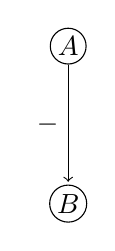
\begin{tikzpicture}[shorten >=1pt,node distance=2cm,on grid]

      \node[state, inner sep=1pt, minimum size=0pt] (A)              {$A$}; 
      \node[state, inner sep=1pt, minimum size=0pt] (B) [below=of A] {$B$}; 
     
        
      \path[->] (A) edge []     node[left]     {$-$}   (B);
    
    \end{tikzpicture}
    \end{minipage}
    
    \end{tabular}
    
    \caption{Пример стратифицированной программы}
    \label{fig:strat}
\end{figure}

\begin{figure}[h]
    \begin{tabular}{p{0.5\textwidth}|p{0.5\textwidth}}
    
    \begin{minipage}{0.4\textwidth}  %listing bloc will have 50% of the line width 
    \begin{lstlisting}
        let A x y = $\neg$B x y
        let B x y = A x y 
        \end{lstlisting}
    \end{minipage}
    
    &
    
    \hspace{2.5cm}
    \begin{minipage}{0.4\textwidth} %figure will have the remaning 40% of the line width
    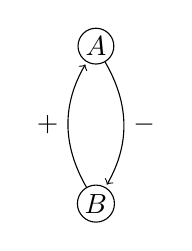
\begin{tikzpicture}[shorten >=1pt,node distance=2cm,on grid]
    
        \node[state, inner sep=1pt, minimum size=0pt] (A)              {$A$}; 
        \node[state, inner sep=1pt, minimum size=0pt] (B) [below=of A] {$B$}; 
     
        \path[->] (A) edge [bend left]     node[right]    {$-$}   (B);
        \path[->] (B) edge [bend left]     node[left]     {$+$}   (A);
    
    \end{tikzpicture}
    \end{minipage}
    
    \end{tabular}
    
    \caption{Пример нестратифицированной программы}
    \label{fig:non-strat}
\end{figure}

Для того, чтобы дать определение стратифицированной реляционной программы,
свяжем с каждой программой ориентированный граф.
Вершинами в данном графе являются отношения.
Между двумя вершинами $A$ и $B$ есть ребро $A \rightarrow B$, 
если отношение $B$ встречается в определении отношения $A$.
Если $B$ встречается в определении $A$ в позитивной форме (т.е. без отрицания), 
то будем помечать ребро меткой $+$, иначе меткой $-$.
Реляционная программа является стратифицированной, если 
в соответствующем графе нет циклов, 
содержащих хотя бы одно ребро с меткой $-$.
На рисунке~\ref{fig:strat} приводится пример стратифицированной программы,
а на рисунке~\ref{fig:non-strat} --- нестратифицированной программы.

Граф стратифицированной программы может быть разбит на компоненты связности
по отношению связности по ребрам с меткой $+$.
Данные компоненты называются \emph{стратами}.
Страты соединены ребрами с меткой $-$.
Определение стратифицированной программы гарантирует, 
что между стратами нет циклических зависимостей.

Применительно к реляционному интерпретатору,
основанному на СПП (раздел~\ref{sec:tls}),
отрицание позволяет проверять недостижимость некоторого состояния.
В рамках данной работы было реализовано расширение 
языка OCanren для поддержки метода конструктивного отрицания (раздел~\ref{sec:negation-impl}).

\subsubsection{Табличная мемоизация}

\label{sec:tabling}

Табличная мемоизация --- это метод оптимизации реляционных программ,
заключающийся в переиспользовании ответов на подзапросы.
Данный метод способен ускорить исполнение запросов к рекурсивным отношениям.
Кроме того, применение мемозации к некоторым отношениям 
позволяет запросам к данным отношениям завершаться за конечное время, 
в то время как аналогичные запросы к немемоизированной версии отношения 
не завершаются.

\begin{figure}[h]
    \begin{tabular}{p{0.6\textwidth}|p{0.4\textwidth}}
    
    \begin{minipage}{0.5\textwidth}
    \begin{lstlisting}[
        % caption={Определение отношения \texttt{reachable$^o$}},
        % label={lst:reachableo}
    ]
    let edge$^o$ x y = 
      (x, y) === ("a", "b") \/
      (x, y) === ("b", "a") \/
      (x, y) === ("b", "d")
    
    let reachable$^o$ x y = 
      (x === y) \/
      fresh (z)
        (edge$^o$ x z) /\ 
        (reachable$^o$ z y)
    \end{lstlisting}
    \end{minipage}
    
    &
    
    % \hspace{2.5cm}
    \begin{minipage}{0.3\textwidth} %figure will have the remaning 40% of the line width
    
    \begin{center}
    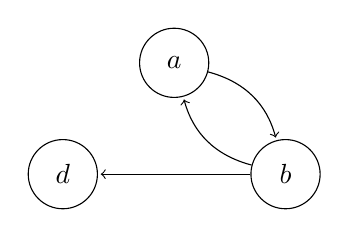
\begin{tikzpicture}[shorten >=1pt,node distance=2cm,on grid]

    \node[state] (s1)                 {$a$}; 
    \node[state] (s2) [below right=of s1]   {$b$};
    \node[state] (s3) [below left =of s1]   {$d$};
    
    \path[->] (s1) edge [bend left]     node[] {}   (s2);
    \path[->] (s2) edge [bend left]     node[] {}   (s1);
    \path[->] (s2) edge []              node[] {}   (s3);
    
    \end{tikzpicture}
    \end{center}
    
    \end{minipage}
    
    \end{tabular}
    
    \caption{Определение отношения достижимости на графе}
    \label{fig:reachable}
\end{figure}

Рассмотрим классический пример.
На рисунке~\ref{fig:reachable} слева показано отношение
\texttt{edge$^o$}, задающее пары связанных вершин в графе, 
и отношение \texttt{reachable$^o$}, 
задающее отношение достижимости на графе.
Справа показано изображение графа, 
соответствующего заданному отношением \texttt{edge$^o$}.
Запрос \texttt{run * (reachable$^o$ "a" q)} 
к немемоизированной версии отношения завершается успехом 
и возвращает бесконечный список ответов 
\texttt{\{q = "a"; q = "b"; q = "d"; q = "a"; q = "b"; q = "d"; ... \}},
в то время как этот же запрос к мемоизированной версии 
возвращает конечный список ответов \texttt{\{q = "a"; q = "b"; q = "d"; \}}.

Системы помеченных переходов (раздел~\ref{sec:tls}) 
также задают граф, а трасса соответствует некоторому пути в графе.
При попытке определить отношение достижимости на СПП 
можно натолкнуться на проблемы аналогичные тем, 
что возникают при определении отношения \texttt{reachable$^o$}.
Таким образом, при написании реляционных интерпретаторов на 
основе СПП наличие поддержки табличной мемоизации 
в реляционном языке становится критически важным.

Табличный метод мемоизации был реализован 
в нескольких версиях языка Prolog~\cite{swift2012xsb, wielemaker2012swi}.
В работе~\cite{byrd2009relational} представлена реализация данного метода 
для языка MiniKanren, втроенного в Scheme.
В рамках данный работы эта реализация была улучшена 
(добавлена поддержка ограничений неэквивалентности и 
использованы более эффективные структуры данных)
и встроена в язык OCanren типобезопасным образом.

\subsection{Реализация языка OCanren}

\label{sec:ocanren-impl}

Для понимания дальнейшего содержания работы,
в частности, реализации расширений OCanren,
необходимо рассмотреть основные идеи, 
лежащие в основе реализации этого языка.

Главная идея заключается в том, чтобы 
встроить интерпретатор реляционного языка в функциональный язык 
с помощью использования монады с выбором (MonadPlus)~\cite{kiselyov2005backtracking, kosarev2016typed}.
OCanren использует реализацию монады с выбором, основанную на ленивых потоках (Streams).

При исполнении запроса происходит поиск ответов.
Использование монады с выбором позволяет закодировать 
чередующийся поиск с возвратом (interleaving search).
Данный вид поиска является полным в отличии от 
применяемого в языках семейства Prolog поиска в глубину (depth-first search).

Каждая ветка поиска поддерживает текущее состояние,
которое кодирует множество ограничений, накопленных в данной ветке.
Состояние кодирует систему консистентных (т.е. выполнимых) ограничений.
Если при добавлении очередного ограничения в состояние
система становится неконсистентной, 
данная ветка поиска может быть отсечена.

Выполнимость ограничений эквивалентности может быть проверена 
с помощью алгоритма унификации~\cite{baader2001unification}.
Алгоритм унификации либо приводит выполнимое ограничение $\unify$ 
в решенную форму (solved form),
либо детектирует невыполнимость.
Решенная форма для ограничений эквивалентности 
это подстановка $\sigma$, т.е. частичная функция, которая ставит в соответствие 
логическим переменным термы $\sigma :: V \rightarrow T$.
Применение данной подстановки к термам делает их синтаксически эквивалентными:
$\sigma(t) = \sigma(u)$.

%% Например, для термов \texttt{Cons(1, _$_{0}$)} и \texttt{Cons(_$_{1}$, Nil)}
%% алгоритм унификации возвращает подстановку 
%% $\sigma = \{\__{0} \mapsto \mbox{\texttt{Nil}}; ~ \__{1} \mapsto \mbox{\texttt{1}}\}$.
%% Для термов \texttt{Cons(1, _$_{0}$)} и \texttt{Nil} такой подстановки не существует,
%% и алгоритм унификации возвращает $\bot$.

\begin{algorithm}
\begin{algorithmic}[1]

\Procedure{Unify}{$\sigma, L$}
\If {$L = \varnothing$} 
  \Return {$\sigma$}
\EndIf
  \State {pick $(t \equiv u) \in L$}
  \State {L := $L \setminus (t \equiv u)$}
  \Switch {$\sigma(t), ~ \sigma(u)$}
    
    % \Comment{Унификация двух конструкторов}
    \Case {$C^n_i(t_1, ..., t_n), ~ C^m_j(u_1, ..., u_m)$}  \label{algo:line:unify-ctor-start}
      \If {$i = j$}
        \State {L := $\{t_1 \equiv u_1, ...~, t_n \equiv u_n\} \cup L$}
      \Else~
        \Return {$\bot$}
      \EndIf
    \EndCase \label{algo:line:unify-ctor-end}
    
    % \Comment{Унификация двух переменных}
    \Case {$x, ~ y$ \textbf{when} $var(x)$ \AND $var(y)$} \label{algo:line:unify-var-var-start}
        \State {$\sigma$ := $\{x \mapsto y\} \cup \sigma$ }
    \EndCase \label{algo:line:unify-var-var-end}
    
    % \Comment{Унификация переменной с термом}
    \Case {$x, ~ t = C^n(t_1, \dots, t_n)$ \textbf{when} $var(x)$} \label{algo:line:unify-var-term-start}
      \If {$x \in Vars(t)$} 
        \Return {$\bot$}
      \Else 
        \State {$\sigma$ := $\{x \mapsto t\} \cup \sigma$ }
      \EndIf
    \EndCase \label{algo:line:unify-var-term-end}
    
  \EndSwitch
  
  \Return Unify($\sigma,L$)
\EndProcedure

\end{algorithmic}
\caption{Алгоритм унификации}
\label{algo:unify}
\end{algorithm}

Псевдокод процедуры унификации представлен в алгоритме~\ref{algo:unify}.
Процедура унификации принимает на вход 
текущую подстановку для переменных $\sigma$ и
список ограничений $\unify \in L$.
Для проверки ограничения $\unify$ 
на вход унификации подаются $\sigma = \emptyset$ и $L = \{\unify\}$.
Результатом работы процедуры является подстановка для переменных $\sigma'$,
если ограничение выполнимо, и $\bot$ иначе.

Разберём, как работает данный алгоритм.
Если список $L$ пуст --- процедура оканчивает работу, возвращая текущую подстановку.
Иначе недетерменированно выбирается одно из ограничений $\unify$.
К термам $t$ и $u$ применяется текущая подстановка и выполняется разбор случаев.
Если в корне двух термов находятся конструкторы 
(строки~\ref{algo:line:unify-ctor-start}-\ref{algo:line:unify-ctor-end})
и эти конструкторы равны, то в $L$ добавляются новые ограничения на 
равенство аргументов конструкторов.
Если конструкторы различны --- алгоритм оканчивается неудачей (возвращается $\bot$).
Если оба терма являются переменными 
(строки~\ref{algo:line:unify-var-var-start}-\ref{algo:line:unify-var-var-end}),
в подстановку добавляются новое связывание
(переменная $x$ связывается с $y$).
Наконец, рассматривается случай, когда один из термов является переменной, 
а в корне другого находится конструктор
(строки~\ref{algo:line:unify-var-term-start}-\ref{algo:line:unify-var-term-end}).
Выполняется проверка, входит 
ли переменная $x$ в терм $t$ (\emph{occurs-check}).
В случае если это так алгоритм заключает, что ограничения невыполнимы.
Иначе переменная $x$ связывается с $t$ в подстановке.
После разбора всех случаев выполняется рекурсивный вызов процедуры унификации
на обновленном множестве $L$ и подстановке $\sigma$.

Проверка ограничения $\diseq$ также выполняется при помощи алгоритма унификации.
Чтобы проверить выполнимость $\diseq$
на вход подается $\sigma = \emptyset$, $L = \{\unify\}$
и проверяется, что в результате процедура возвращает 
либо $\bot$, либо непустую подстановку $\sigma \neq \emptyset$.

\section{Расширения OCanren}

Далее приводится описание расширений языка OCanren, реализованных в ходе данной работы. 

\subsection{Конструктивное отрицание}

\label{sec:negation-impl}

В данном разделе будет представлена реализация расширения OCanren 
для поддержки метода конструктивного отрицания.
Сперва будет представлена семантика конструктивного отрицания (раздел~\ref{sec:negation-semantics}). 
Будет показано, что для конструктивного отрицания
необходимо добавить в язык поддержку 
двух новых видов ограничений $\antisubs$ 
и $\qunify$.
В разделах~\ref{sec:negation-antisubs} и~\ref{sec:negation-qunify} 
будут представлены алгоритмы для проверки выполнимости данных ограничений.
% Наконец, в разделе~\ref{sec:negation-op} приводится 
% описание реализации оператора отрицания.

\subsubsection{Семантика конструктивного отрицания}

\label{sec:negation-semantics}

Для того, чтобы определить семантику конструктивного отрицания
будем рассматривать процесс ответа на запрос как процедуру трансляции
в логическую формулу~\cite{przymusinski1989constructive}.
Предположим, что определение отношения содержит только ``положительные'' 
вхождения других отношений и не содержит отношений неэквивалентности 
(будем называть такую программу \emph{положительной}).
В таком случае, множество ответов на запрос к такой программе 
соответствует формуле~\ref{eq:query-positive}.

\begin{equation}
E_{+} = \exists~\overline{x}.\bigvee_{i=1}^{N}~\bigwedge_{j=1}^{M_i}{t_{ij} \equiv u_{ij}}
\label{eq:query-positive}
\end{equation}

Таким образом, множество ответов на запрос к отрицанию данного отношения 
должно соответствовать отрицанию формулы~\ref{eq:query-positive} 
(показано в формуле~\ref{eq:query-negation-positive}).
Заметим, что формула~\ref{eq:query-negation-positive} содержит 
ограничения неэквивалентности на термы, 
которые могут содержать универсально квантифицированные переменные,
т.е. ограничения вида $\antisubs$.
Данные ограничения сводятся к обычным ограничениям неэквивалентности 
$\diseq$ в случае когда список 
универсально квантифицированных переменных $\overline{x}$ пуст.

\begin{equation}
\neg E_{+} = 
  \forall~\overline{x}.\bigwedge_{i=1}^{N}~\bigvee_{j=1}^{M_i}{t_{ij} \not\equiv u_{ij}}
\label{eq:query-negation-positive}
\end{equation}

Перейдем к рассмотрению отношений, которые также могут содержать как 
``положительные'' так и ``отрицательные'' вхождения других отношений.
Будем рассматривать только стратифицированные программы (раздел~\ref{sec:negation}).
В этом случае, можно разбить реляционную программу на страты,
выполнить топологическую сортировку страт и 
строить ответ на запрос поэтапно, начиная с последней страты в порядке сортировки.

По построению, последней страте соответствует некоторое ``положительное'' отношение,
т.е. в определении данного отношения не встречаются ``отрицательные'' вхождения других отношений. 
Это значит, что ответу на запрос к данному отношению соответствует 
логическая формула~\ref{eq:query-positive}.
Рассмотрим отрицание данной формулы (формула~\ref{eq:query-negation-positive}) 
и подставим его на место всех ``отрицательных'' вхождений
данного отношения в предыдущей страте.
После трансляции предыдущей страты получим формулу~\ref{eq:query-strat}.

\begin{equation}
E = \exists~\overline{x}.\bigvee_{i=1}^{N}~
  ((\bigwedge_{j=1}^{M_i}{t_{ij} \equiv u_{ij}}) 
  \wedge
  ({\forall\overline{y}.\bigwedge_{k=1}^{L_i}~\bigvee_{l=1}^{Q_k}{p_{kl} \not\equiv u_{kl}}})
  )
\label{eq:query-strat}
\end{equation}

В результате отрицания формулы~\ref{eq:query-strat}
получим формулу~\ref{eq:query-negation-strat}.

\begin{equation}
 \neg E = \forall~\overline{x}.\bigwedge_{i=1}^{N}~
    ((\bigvee_{j=1}^{M_i}{t_{ij} \not\equiv u_{ij}}) 
    \vee
    ({\exists\overline{y}.\bigvee_{k=1}^{L_i}~\bigwedge_{l=1}^{Q_i}{p_{kl} \equiv u_{kl}}})
    )
\label{eq:query-negation-strat}
\end{equation}

Формула~\ref{eq:query-negation-strat} содержит отношения эквивалентности на термах, 
которые могут содержать свободные переменные, а также как экзистенциально 
так и универсально квантифицированные переменные, 
т.е. ограничения вида $\qunify$.
Отношения эквивалентности данного вида не могут быть решены 
обычным алгоритмом унификации.
Тем не менее, существует расширение алгоритма унификации,
которое позволяет решать подобные ограничения~\cite{liu1999constructive}.
Более подробное описание данного алгоритма унификации приведено в разделе~\ref{sec:negation-qunify},
здесь лишь отметим, что данный алгоритм позволяет 
получить по формуле вида $\qunify$ 
формулу вида $\exists{y'}.t' \equiv u'$.
Таким образом, формулу~\ref{eq:query-negation-strat} можно переписать,
избавившись от ограничений вида $\qunify$,
как показано в формуле~\ref{eq:query-negation-strat-simpl}.

\begin{equation}
\neg E = \bigwedge_{i=1}^{N}~
    (({\exists\overline{y'}.~\bigvee_{k=1}^{L'_i}~\bigwedge_{l=1}^{Q'_i}{p'_{kl} \equiv u'_{kl}}})
    \vee
    \forall~\overline{x}.
    (\bigvee_{j=1}^{M_i}{t_{ij} \not\equiv u_{ij}}))
\label{eq:query-negation-strat-simpl}
\end{equation}

Раскрыв внешнюю конъюнкцию в данной формуле по правилу дистрибутивности,
получим формулу, аналогичную по форме формуле~\ref{eq:query-strat}.
Данную формулу можно подставить в предыдущую в порядке сортировки страту и повторить процесс.
Итеративно повторив этот процесс для всех страт, получим в итоге формулу,
соответствующую исходному запросу.

%% \subsubsection{Решение ограничений \texorpdfstring{$\antisubs$}{анти-обобщения}}
\subsubsection{Решение ограничений анти-обобщения}

\label{sec:negation-antisubs}

Вернемся к рассмотрению ограничений вида $\antisubs$.
Необходимо предоставить процедуру, которая сможет проверить выполнимость данных ограничений.
Для того чтобы предоставить такой алгоритм, 
мы обобщили алгоритм для проверки выполнимости 
обычных ограничений неэквивалентности $\diseq$.

Прежде, чем переходить к описанию алгоритма, заметим, 
что ограничение $\antisubs$ не выполнимо тогда и только тогда, 
когда существует подстановка для переменных $\overline{x}$,
применение которой к термам $t$ и $u$ делает их 
синтаксически эквивалентными (формуа~\ref{eq:antisubs-sat}).
Таким образом, для опровержения выполнимости $\antisubs$
достаточно предъявить такую подстановку.

\begin{equation}
\forall{\overline{x}}.t \not\equiv u \Leftrightarrow \neg \exists{x}. t \equiv u    
\label{eq:antisubs-sat}
\end{equation}

Теперь обобщим алгоритм проверки выполнимости ограничений неэквивалентности таким образом,
чтобы он также пытался построить данную подстановку.
Напомним, что алгоритм для проверки ограничения $\diseq$
выполняет унификацию термов $t$ и $u$, 
т.е. возвращает либо подстановку $\sigma : \sigma(t) = \sigma(u)$,
либо $\bot$ если термы не унифицируются.
Если термы унифицируются в пустой подстановке $\sigma = \emptyset$,
то ограничение не выполнимо, иначе оно выполнимо.

Для того, чтобы проверять ограничения вида $\antisubs$,
достаточно лишь слегка модифицировать алгоритм.
В случае, если унификация термов $t$ и $u$ вернула 
непустую подстановку $\sigma$, 
необходимо проверить, связывает ли эта подставновка
только универсально квантифицированные переменные $\overline{x}$.
Если это так, то мы доказали невыполнимость ограничения 
и предъявили контрпример --- подстановку $\sigma$, 
такую что $Dom(\sigma) \subseteq \overline{x}$ и 
$\sigma(t) = \sigma(u)$.
Иначе ограничение выполнимо.

%% \subsubsection{Решение ограничений \texorpdfstring{$\qunify$}{эквивалентности с кванторами}}
\subsubsection{Решение ограничений эквивалентности с кванторами}

\label{sec:negation-qunify}

Перейдем к рассмотрению ограничений $\qunify$.
Для проверки выполнимости данных ограничений 
мы воспользуемся модификацией алгоритма унификации\cite{liu1999constructive}.
Модифицированный алгоритм позволяет обрабатывать 
встречающиеся в термах универсально и экзистенциально квантифицированные переменные
при условии, что квантор всеобщности предшествует квантору существования
(это как раз случай ограничений $\qunify$).
Заметим, что помимо квантифицированных переменных в термах также могут 
присутствовать свободные переменные.

Алгоритм~\ref{algo:qunify} содержит псевдокод модифицированной процедуры унификации.
Процедура принимает на вход множество универсально квантифицированных переменные $U$,
множество экзистенциально квантифицированных переменных $E$,
текущую подстановку для переменных $\sigma$ и
список ограничений $\unify \in L$.
Переменные $x \not\in U \cup E$ считаются свободными.
Для проверки решения ограничения $\qunify$ 
на вход унификации подаются $U = \overline{x}$, 
$E = \overline{y}$, $\sigma = \emptyset$ и $L = \{\unify\}$.
Результатом работы процедуры является подстановка для переменных $\sigma'$,
если ограничение выполнимо, и $\bot$ иначе.

\begin{algorithm}
\begin{algorithmic}[1]

\Procedure{Unify}{$U, E, \sigma, L$}
\If {$L = \varnothing$} 
  \Return {$\sigma$}
\EndIf
  \State {pick $(t \equiv u) \in L$}
  \State {L := $L \setminus (t \equiv u)$}
  \Switch {$\sigma(t), ~ \sigma(u)$}
    
    % \Comment{Унификация двух конструкторов}
    \Case {$C^n_i(t_1, ..., t_n), ~ C^m_j(u_1, ..., u_m)$} 
      \If {$i = j$}
        \State {L := $\{t_1 \equiv u_1, ...~, t_n \equiv u_n\} \cup L$}
      \Else~
        \Return {$\bot$}
      \EndIf
    \EndCase
    
    % \Comment{Унификация переменной с термом}
    \Case {$x, ~ y$ \textbf{when} $var(x)$ \AND $var(y)$} \label{algo:line:qunify-var-var-start} 
      \If {$x \in U$ \AND $y \in U$}
        \Return {$\bot$}
      \ElsIf {$x \in E$} 
        % \State {C := Replace(C, x, y)}
        \State {$\sigma$ := $\{x \mapsto y\} \cup \sigma$ }
      \ElsIf {$y \in E$}
        \State {$\sigma$ := $\{y \mapsto x\} \cup \sigma$ }
      % \Comment{$x, y$ --- свободные переменные}
      \ElsIf {$x \in U$ \textbf{or} $y \in U$}
        \Return {$\bot$}
      \Else
        \State {$\sigma$ := $\{x \mapsto y\} \cup \sigma$ } \label{algo:line:qunify-var-var-end}
      \EndIf
    \EndCase
    
    % \Comment{Унификация переменной с термом}
    \Case {$x, ~ t = C^n(t_1, \dots, t_n)$ \textbf{when} $var(x)$} \label{algo:line:qunify-var-term-start} 
      \If {$x \in U$ \textbf{or} $x \in Vars(t)$} 
        \Return {$\bot$}
      \ElsIf {$x \in E$}
        \State {$\sigma$ := $\{x \mapsto t\} \cup \sigma$ }
      % \Comment{$x$ --- свободная переменная}
      \ElsIf {$Vars(t) \cap U = \varnothing $} 
        \State {$z_1, \dots, z_n$ --- свежие свободные переменные}
        \State {$\sigma$ := $\{x \mapsto C^n(z_1, \dots, z_n)\} \cup \sigma$ }
        \State {L := $\{z_1 \equiv t_1, \dots, z_n \equiv t_n\} \cup L$}
      \Else~ 
        \Return {$\bot$} \label{algo:line:qunify-var-term-end}
      \EndIf
    \EndCase
    
  \EndSwitch
  
  \Return Unify($U, E, \sigma,L$)
\EndProcedure

\end{algorithmic}
\caption{Расширенный алгоритм унификации}
\label{algo:qunify}
\end{algorithm}

Как можно видеть, алгоритм~\ref{algo:qunify} очень похож 
на стандартный алгоритм унификации.
Рассмотрим главные отличия.

Если оба терма являются переменными 
(строки~\ref{algo:line:qunify-var-var-start}-\ref{algo:line:qunify-var-var-end})
рассматривается несколько случаев.
Если обе переменные универсально квантифицированны, алгоритм возвращает $\bot$.
Если одна из переменных экзистенциально квантифицированна, 
в подстановку добавляется связывание для этой переменной.
Иначе одна из переменных является свободной.
Если вторая переменная при этом универсально квантифицирована, то нужно вернуть $\bot$.
Если и вторая переменная свободна, 
в подстановку добавляется новое связывание 
для одной из переменных (неважно, $x$ или $y$). 

Если один из термов является переменной, 
а в корне другого терма конструктор, 
вновь рассматривается несколько случаев
(строки~\ref{algo:line:qunify-var-term-start}-\ref{algo:line:qunify-var-term-end}).
Если переменная универсально квантифицирована
или она встречается в терме $t$ (occurs check),
алгоритм возвращает $\bot$.
Если переменная экзистенциально квантифицирована,
в подстановку добавляется связывание для неё.
Если переменная свободна и терм не содержит универсально квантифицированных переменных, 
то алгоритм создает $n$ новых свободных переменных $z_1, \dots, z_n$ 
по числу аргументов конструктора $C^n$.
В подстановке переменная связывается с термом $C^n(z_1, \dots, z_n)$, 
а в множество ограничений $L$ добавляются 
ограничения эквивалентности для новых переменных 
и соответствующих подтермов $t$. 

Обратим внимание, что в получившейся подстановке $\sigma'$
нет связываний для унивесально квантифицированных переменных,
а все свободные переменные связаны с термами, 
не содержащими унивесально квантифицированные переменные.
Это значит, что в результате работы алгоритма 
мы свели ограничение $\qunify$ к набору ограничений 
$\exists{\overline{y'}.x \equiv t}$,
которые выполнимы по построению. 

\subsection{Табличная мемоизация}

\label{sec:tabling-impl}

Как уже было сказано в разделе~\ref{sec:tabling},
идея метода табличной мемоизации заключается в 
сохранении и переиспользовании ответов на запрос.
Для этого, с каждым мемоизированным отношением связывается таблица,
в которой ключом является запрос 
(т.е. набор переданных аргументов отношения),
а значением --- список ответов на данный запрос.
Если в ходе исполнения программы вновь будет сделан запрос,
эквивалентный некоторому более раннему, 
ответы на данный запрос будут извлечены из таблицы.

\begin{figure}[!htb]
\centering

\tikzstyle{block} = [rectangle, draw,
    text width=8em, text centered, rounded corners, on grid]

\tikzset{node distance = 2cm and 2cm}

\tikzstyle{line} = [draw, -latex']

\tikzstyle{line-text} = [text width=6em, text centered, inner sep=0,outer sep=0]


\begin{tikzpicture}[yscale=0.8,xscale=0.8]
    % Place nodes
    \node [block]                           (query)         {Запрос к отношению};
    \node [block, below of=query]           (abs)           {Абстрагирование аргументов};
    \node [block, below of=abs]             (search)        {Поиск аргументов в таблице};
    \node [block, below left = of search]   (query-next)    {Запрос следующего ответа};
    \node [block, below = of query-next]    (search-answ)   {Поиск ответа в таблице};
    \node [block, below = of search-answ]   (update)        {Добавление ответа в таблицу};
    \node [block, below right = of search]  (extract)       {Извлечение ответов из таблицы};
    \node [block, below = of extract]       (concretize)    {Конкретизация ответов};
    
    
    \path [line] (query)    --      (abs);
    \path [line] (abs)      --      (search);
    \path [line] (extract)  --      (concretize);
    
    \path [line] (search)           -|      node [line-text, left]  {Аргументы не найдены}  (query-next);
    \path [line] (query-next)       -- node [line-text, left]       {Ответ получен}         (search-answ);
    \path [line] (search-answ)      -- node [line-text, left]       {Ответ не найден}       (update);
    \path [line] (search)           -| node [line-text, right]      {Аргументы найдены}     (extract);
    
    \path [line] (search-answ.west) -- +(-0.8,0) |- node [line-text, left, text width=6em, pos=0.25]    {Ответ найден} (query-next);
    \path [line] (query-next)       -- +(2.5,0)  |- node [line-text, right, pos=0.225]                  {Ответов больше нет} (concretize);
    
    
\end{tikzpicture}

\caption{Блок-схема алгоритма табличной мемоизации}
\label{fig:tabling-algo}
\end{figure}

Возникает вопрос, какие запросы считать эквивалентными?
Мы полагаем, что два запроса эквиваленты,
если наборы их аргументов \emph{альфа-эквиваленты},
т.е. синтаксически равны с точностью до переименования переменных.
Более формально: 
$t =_{\alpha} u \Leftrightarrow \exists \sigma. \sigma(t) = \sigma(u) \wedge Dom(\sigma) \subseteq V$.

Табличная мемоизация добавляет в OCanren два новых примитива --- \texttt{tabled} и \texttt{tabledrec},
которые позволяют получить мемоизированную версию отношения типобезопасным образом.
Примитив \texttt{tabled} используется для мемоизации нерекурсивных отношений.
При необходимости применить мемоизацию к рекурсивному отношению, 
пользователю необходимо немного модифицировать определение отношения.
Требуется абстрагироваться от рекурсивного вызова,
сделав его первым параметром отношения.
После этого необходимо применить к полученному отношению примитив \texttt{tabledrec}.
Можно видеть, что \texttt{tabledrec} является своего рода комбинатором неподвижной точки.

\begin{figure}[thp]
\begin{center}
\begin{tabular}{c}
\begin{lstlisting}
let edge$^o$ x y = 
  (x === 'a') /\ (y === 'b')
  \/
  (x === 'b') /\ (y === 'a')
  \/
  (x === 'b') /\ (y === 'd')

let edge$^o_{tabled}$ = tabled edge$^o$ 
\end{lstlisting}
\end{tabular}
\end{center}
\caption{Пример мемоизации нерекурсивного отношения}
\label{lst:tabled}
\end{figure}

\begin{figure}[thp]
\begin{center}
\begin{tabular}{c}
\begin{lstlisting}
let reachable$^o_{norec}$ reachable$^o_{rec}$ x y = 
  (edge$^o$ x y)
  \/
  fresh (z)
    (edge$^o$ x z) /\ (rec$^o$ z y)
    
let reachable$^o_{tabled}$ = tabledrec reachable$^o$ 
\end{lstlisting}
\end{tabular}
\end{center}
\caption{Пример мемоизации рекурсивного отношения}
\label{lst:tabledrec}
\end{figure}

Схема алгоритма табличной мемоизации представлена на рис. \ref{fig:tabling-algo}.

При выполнении запроса к отношению сначала выполняется \emph{абстракция} аргументов. 
Абстракция аргументов позволяет уменьшить размер таблицы для хранения 
аргументов и списка ответов --- несколько запросов с различными аргументами
потенциально могут быть абстрагированы до одного запроса.
Сильная абстракция может привести 
к множеству повторяющихся вычислений на этапе конкретизации 
(подробнее о конкретизации ниже).
Кроме того, сильная абстракция может привести 
к тому, что запросы к рекурсивным отношениям не смогут завершиться за конечное время.
Таким образом, при абстракции необходим разумный компромисс 
между экономией памяти (чем сильнее абстракция, тем меньше запросов храниться в таблице)
и временем работы и терменируемостью запросов.
В нашей реализации при абстракции аргументов отбрасывается 
информация об ограничениях неэквивалентности
(по соображениям простоты реализации, следуя работе~\cite{schrijvers2008tchr}).

Полученный после абстракции список аргументов используется как ключ
для поиска записи об эквивалентном запросе в таблице. 
В качестве структуры данных для хранения множества используется хеш-таблица. 
Перед вычислением хеша логического терма выполняется переименование 
всех переменных в порядке обхода терма в глубину. 
Это необходимо для того, чтобы альфа-эквивалентые термы имели одинаковый хеш.

В случае, когда запись не была найдена в таблице, 
необходимо выполнить запрос к немемоизированной версии отношения, чтобы получить ответы.
Для каждого полученного ответа выполняется проверка, 
не был ли данный ответ добавлен в таблицу ранее.
Если такой ответ встречается впервые, он добавляется в таблицу.

В случае, когда запись была найдена, т.е. запрос к отношению
с соответствующими аргументами уже был выполнен ранее,
необходимо извлечь полученные ранее ответы из таблицы.

Перед возвращением списка ответов необходимо выполнить их конкретизацию.
Напомним, что табличный алгоритм начинается с абстракции аргументов вызова.
Абстракция может удалить некоторую информацию об аргументах,
чтобы привести их к более общему виду.
Другими словами, полученные ответы являются ответами не на исходный запрос,
а на его абстрагированную версию.
Чтобы получить ответ на исходный запрос необходимо "скомбинировать" информацию об аргументах,
потерянную на стадии абстракции и полученные ответы.
Заметим, что возможна ситуация, при которой некоторые ответы окажутся отброшены
как не удовлетворяющие исходному запросу.
Таким образом, хотя информации об ограничениях неэквивалентности была отброшена на стадии абстракции, 
на этапе конкретизации происходит проверка совместимости ограничений с полученными ответами.

\section{Реляционный интерпретатор}

В данном разделе описан реляционный интерпретатор 
для императивного языка программирования с многопоточностью. 
Для задания семантики императивного языка мы используем системы помеченных переходов. 
Сначала мы определим основные типы данных, необходимые для СПП.
Затем мы покажем, как имея отношение перехода step$^o$ 
построить отношение достижимости на СПП reachable$^o$.
При помощи данного отношения будет определено 
отношение eval$^o$ для вычисления программы,
а также отношение invariant$^o$ для проверки инвариантов программы.

Для того, чтобы поддержать несколько моделей памяти,
мы будем представлять систему переходов как 
пару двух подсистем --- подсистемы потоков и подсистемы памяти. 
Подсистема потоков отвечает за 
хранение локальных переменных потока и его команд,
а также за планирование исполнения
(т.е. выбор потока для исполнения следующей команды).
Подсистема памяти описывает эффекты обращений к общей памяти, 
такие как чтения и записи разделямых переменных.
Таким образом, изменяя реализации подсистемы памяти,
можно получить интерпретаторы, работающие с различными моделями памяти.

\subsection{Реляционные системы помеченных переходов}

Напомним, что система помеченных переходов (СПП) --- это 
четвёрка $(S, I, L, R)$, где $S$ --- это множество состояний, 
$I \subseteq S$ --- множество начальных состояний,
$L$ --- множество меток, а $R \subseteq L \times S \times S$ --- отношение перехода.
СПП тривиальным образом кодируются в реляционную программу.
Необходимо определить типы данных \texttt{State} и \texttt{Label},
а также отношение перехода \texttt{step$^o$} (листинг~\ref{lst:tls-basics}).

\begin{figure}[thb]
\begin{minipage}{\linewidth}
\begin{lstlisting}[
  caption={Основные компоненты реляционной СПП},
  label={lst:tls-basics}
]
type state

type label

val step$^o$ :: label $\times$ state $\times$ state
\end{lstlisting}
\end{minipage}
\end{figure}

\begin{figure}[thb]
\begin{minipage}{\linewidth}
\begin{lstlisting}[
  caption={Определение отношения \texttt{reachable$^o$} для СПП},
  label={lst:tls-reachable}
]
let reachable$^o$ p$^o$ s s' = 
  let reachable$^o_{norec}$ reachable$^o_{rec}$ s s'' = 
    ((p$^o$ s) /\ (s === s'')) \/
    fresh (s')
      (step$^o$ s s') /\ 
      (reachable$^o_{rec}$ s' s'')
  in
  let reachable$^o_{tabled}$ = 
    tabledrec$_2$ reachable$^o_{norec}$
  in
  reachable$^o_{tabled}$ s s'
  
\end{lstlisting}
\end{minipage}
\end{figure}

\begin{figure}[thb]
\begin{minipage}{\linewidth}
\begin{lstlisting}[
  caption={Определение отношения \texttt{eval$^o$} для СПП},
  label={lst:tls-eval}
]
let eval$^o$ t t' = reachable$^o$ terminal$^o$ t t'
\end{lstlisting}
\end{minipage}
\end{figure}

Далее можно определить отношение достижимости \texttt{reachable$^o$} (листинг~\ref{lst:tls-reachable}),
принимающее предикат p$^o$ и 
связывающее состояние \texttt{s} с некоторым достижимым состоянием \texttt{$s^\prime$},
на котором выполняется p$^o$.
Для того, чтобы избежать проблем, упомянутых в разделе~\ref{sec:tabling},
необходимо применить табличную мемоизацию (раздел~\ref{sec:tabling-impl}).

Передав в качестве p$^o$ отношение \texttt{terminal$^o$},
задающее множество терминальных состояний СПП,
получим отношение \texttt{eval$^o$} (листинг~\ref{lst:tls-eval}), 
связывающее состояние \texttt{s} с достижимым терминальным состоянием \texttt{s'}.

Наконец, можно также определить 
отношение \texttt{invariant$^o$} (листинг~\ref{lst:tls-invariant}), 
предназначенное для проверки инвариантов программ.
Данное отношение принимает в качестве аргументов
одноместное отношение \texttt{safe$^o$},
задающее множество безопасных состояний 
(т.е. тех состояний, в которых инвариант выполняется),
а также начальное состояние \texttt{s}.
Отношение \texttt{invariant$^o$} выполняется 
если все состояния, достижимые из данного, являются безопасными. 
Иначе отношение нарушается.
Обратим внимание, что в определении \texttt{invariant$^o$}
фигурирует применение оператора отрицания.
Важно, что оператор использует метод конструктивного отрицания (раздел~\ref{sec:negation}).
Применение метода ``отрицание как неудача'' некорректно в случае, 
когда начальное состояние содержит свободные переменные.

\begin{figure}[thb]
\begin{minipage}{\linewidth}
\begin{lstlisting}[
  caption={Определение отношения \texttt{invariant$^o$} для СПП},
  label={lst:tls-invariant}
]
let invariant$^o$ safe$^o$ t = $\neg$ (
  fresh (t')
    (reachableo$^o$ $\neg$safe$^o$ t t')
)
\end{lstlisting}
\end{minipage}
\end{figure}

\subsection{Описание языка}

Мы реализовали минималистичный императивный язык программирования, 
способный моделировать поведение многопоточных программ.
Грамматика языка представлена на рисунке~\ref{fig:implang-syntax}.
Язык состоит из выражений и набора стандартных для 
императивных языков операторов, 
в том числе оператора присваивания, условного оператора,
цикла с предусловием и цикла с постусловием.

\begin{figure}[hbt]
\begin{minipage}{\linewidth}

\[
\begin{array}{rcl}
Val         & = &   \mathbb{Z}                                  \\
Reg         & = &   \{r_1, r_2, r_3, \dots\}                    \\
Loc         & = &   \{x, y, z, \dots\}                          \\
Uop         & = &   -                                           \\
Bop         & = &   + ~|~ - ~|~ * ~|~ /                         \\
MO          & = &   rlx ~|~ rel ~|~ acq ~|~ relacq ~|~ sc       \\
Expr        & = &   Val ~|~ Reg                                 \\
            & | &   Uop~Expr                                     \\
            & | &   Expr~Bop~Expr                                \\
Stmt        & = &   Reg := Expr                                 \\
            & | &   Reg := [Loc]_{MO}                            \\
            & | &   [Loc]_{MO} := Expr                            \\
            & | &   Reg := CAS_{(mo_1, mo_2)}(Loc, Expr, Expr)   \\
            & | &   \keyword{skip}                               \\
            & | &   Stmt;~Stmt                                   \\
            & | &   \keyword{if}~Expr~\keyword{then}~Stmt~\keyword{else}~Stmt~\keyword{fi}       \\
            & | &   \keyword{while}~Expr~\keyword{do}~Stmt~\keyword{od}                          \\
            & | &   \keyword{repeat}~Stmt~\keyword{until}~Expr                                  
\end{array}
\]

\end{minipage}
\caption{Синтаксис императивного языка}
\label{fig:implang-syntax}
\end{figure}

Отметим некоторые особенности языка.
Язык различает множество локальных переменных $Reg$ 
и множество разделяемых переменных $Loc$.
Операция чтения разделяемой переменной относится к операторам, 
а не выражениям, так как чтение такой переменной может 
модифицировать внутренее состояние памяти. 
Также в языке присутствует операция атомарного сравнения с обменом
(Compare-And-Swap, CAS).
Данная операция атомарно выполняет чтение значения разделяемой переменной,
сравнивает её с ожидаемым значением (второй аргумент CAS).
Если значения совпали, то CAS заменяет значение переменной на желаемой 
(третий аргумент) и возвращает \texttt{true}, 
иначе значение не изменяется и команда возвращает \texttt{false}.

По аналогии с языком C/C++11 
все операции с разделяемыми переменными 
аннотированы модификатором доступа ($MO$).
Модификатор доступа определяет набор ограничений, 
накладываемых на возможность переупорядочивания 
инструкций в слабых моделях памяти.
На значениях типа $MO$ определено отношение порядка
$mo_1 \sqsubseteq mo_2$, которое означает, что 
$mo_2$ является более строгим модификатором 
и накладывает больше ограничений на переупорядочивание инструкций.
Как и в C/C++11 мы различаем три уровня доступа для операций чтения
$rlx \sqsubseteq acq \sqsubseteq sc$;
три уровня доступа для операций записи
$rlx \sqsubseteq rel \sqsubseteq sc$;
и три уровня доступа для операций чтения-модификации-записи
$rlx \sqsubseteq relacq \sqsubseteq sc$.
Заметим, что операция CAS проаннатирована двумя модификаторами доступа,
первый из которых применяется в случае неудачи, второй в случае успеха.

\subsection{Подсистема потоков}

Опишем подсистему потоков.
Состояние подсистемы потоков состоит из списка потоков,
каждый из которых содержит код программы данного потока, 
а также хранилище локальных переменных (рис.~\ref{fig:thread-subsys-def}).

\begin{figure}[thb]
\begin{minipage}{\linewidth}

\[
\begin{array}{rcl}
RegStorage      & = &   Reg \rightarrow Val      \\
Thread          & = &   Stmt \times RegStorage   \\
ThreadSystem    & = &   Tid \rightarrow Thread
\end{array}
\]

\end{minipage}
\caption{Описание подсистемы потоков}
\label{fig:thread-subsys-def}
\end{figure}

\begin{figure}[!thb]
\begin{minipage}{\linewidth}

\small
       
    \begin{center}
    \AxiomC{$a = R(x, mo, v)$}
    \RightLabel{Load}
    \UnaryInfC{$
        \anglebr{r := [x]_{mo}, s} 
        \xrightarrow[]{a} 
        \anglebr{\keyword{skip}, s[r \mapsto v]}
    $}
    \DisplayProof
    \end{center}

    \begin{center}
    \AxiomC{$a = W(x, mo, v)$}
    \AxiomC{$s(e) = v$}
    \RightLabel{Store}
    \BinaryInfC{$
        \anglebr{[x]_{mo} := e, s}
        \xrightarrow[]{a}
        \anglebr{\keyword{skip}, s}
    $}
    \DisplayProof
    \end{center}
    
    \begin{center}
        \AxiomC{$a = RMW(x, mo_2, v_{r}, v_{w})$}
        \AxiomC{$s(e_{r}) = v_{r}$}
        \AxiomC{$s(e_{w}) = v_{w}$}
        \RightLabel{CAS-Success}
        \TrinaryInfC{$
            \anglebr{r := \keyword{CAS}_{mo_1, mo_2}(x, e_{r}, e_{w}), s} 
            \xrightarrow[]{a} 
            \anglebr{\keyword{skip}, s[r \mapsto 1]}
        $}
        \DisplayProof
    \end{center}
    
    \begin{center}
        \AxiomC{$a = R(x, mo_1, v)$}
        \AxiomC{$s(e_{r}) = v_{r}$}
        \AxiomC{$v \neq v_{r}$}
        \RightLabel{CAS-Fail}
        \TrinaryInfC{$
            \anglebr{r := \keyword{CAS}_{mo_1, mo_2}(x, e_{r}, e_{w}), s} 
            \xrightarrow[]{a} 
            \anglebr{\keyword{skip}, s[r \mapsto 0]}
        $}
        \DisplayProof
    \end{center}

    \begin{center}
    \AxiomC{}
    \RightLabel{Skip}
    \UnaryInfC{$
        \anglebr{\keyword{skip}; p, s} 
        \xrightarrow[]{\epsilon} 
        \anglebr{p, s}
    $}
    \DisplayProof
    \end{center}

    \begin{center}
    \AxiomC{$\anglebr{p_1, s} \xrightarrow[]{\epsilon} \anglebr{p'_1, s'}$}
    \RightLabel{Seq}
    \UnaryInfC{$
        \anglebr{p_1; p_2, s} 
        \xrightarrow[]{\epsilon} 
        \anglebr{p_1'; p2, s'}
    $}
    \DisplayProof
    \end{center}

    \begin{center}
    \AxiomC{$s(e) = v$}
    \RightLabel{Assign}
    \UnaryInfC{$
        \anglebr{r := e, s} 
        \xrightarrow[]{\epsilon} 
        \anglebr{\keyword{skip}, s[r \mapsto v]}
    $}
    \DisplayProof
    \end{center}
    
    \begin{center}
    \AxiomC{$s(e) \neq 0$}
    \RightLabel{If-True}
    \UnaryInfC{$
        \anglebr{\keyword{if} ~ e ~ \keyword{then} ~ p_1 ~ \keyword{else} ~ p_2 ~\keyword{fi}, s} 
        \xrightarrow[]{\epsilon} 
        \anglebr{p_1, s}
    $}
    \DisplayProof
    \end{center}
    
    \begin{center}
    \AxiomC{$s(e) = 0$}
    \RightLabel{If-False}
    \UnaryInfC{$
        \anglebr{\keyword{if} ~ e ~ \keyword{then} ~ p_1 ~ \keyword{else} ~ p_2 ~\keyword{fi}, s} 
        \xrightarrow[]{\epsilon} 
        \anglebr{p_2, s}
    $}
    \DisplayProof
    \end{center}
    
    \begin{center}
    \AxiomC{}
    \RightLabel{While}
    \UnaryInfC{$
        \anglebr{\keyword{while} ~ e ~ \keyword{do} ~ p ~ \keyword{od}, s} 
        \xrightarrow[]{\epsilon} 
        \anglebr{\keyword{if} ~ e ~ \keyword{then} ~ (p; \keyword{while} ~ e ~ \keyword{do} ~ p ~ \keyword{od}) ~ \keyword{else} ~ \keyword{skip}, s}
    $}
    \DisplayProof
    \end{center}
    
    \begin{center}
    \AxiomC{}
    \RightLabel{Repeat}
    \UnaryInfC{$
        \anglebr{\keyword{repeat} ~ p ~ \keyword{until} ~ e, s} 
        \xrightarrow[]{\epsilon} 
        \anglebr{p; \keyword{while} ~ !e ~ \keyword{do} ~ p ~ \keyword{od}, s}
    $}
    \DisplayProof
    \end{center}

\end{minipage}    
\caption{Отношение перехода для потока}
\label{fig:thread-rules}
\end{figure}

\begin{figure}[thb]

\small
    
    \begin{center}
    \AxiomC{$\anglebr{p, s} \xrightarrow[]{a} \anglebr{p', s'}$}
    \UnaryInfC{$
        t[i \mapsto \anglebr{p, s}]
        \xrightarrow[]{i:a} 
        t[i \mapsto \anglebr{p', s'}]
    $}
    \DisplayProof
    \end{center}


\caption{Отношение перехода для подсистемы потоков}
\label{fig:thread-subsys-rules}
\end{figure}

Отношение перехода для одного потока 
связывает два последовательных состояния потока и метку действия.
Допускаются следующие действия: 
$R(x, mo, v)$ --- чтение из разделяемой переменной $x$ 
значения $v$ с модификатором доступа $mo$;
$W(x, mo, v)$ --- запись в разделяемую переменную $x$
значения $v$ с модификатором доступа $mo$;
$RMW(x, mo, v_r, v_w)$ (Read-Modify-Write) --- операция чтения-модификации-записи
в разделяемую переменную $x$ значения $v_w$ с ожидаемым значением $v_r$
и модификатором доступа $mo$. 
Отношение перехода для одного потока 
определяется набором правил, представленных на рис.~\ref{fig:thread-rules}.
Отношение перехода для подсистемы потоков недетерменированно 
выбирает пару из идентификатора и потока и выполняет переход 
для выбранного потока (рис.\ref{fig:thread-subsys-rules}).

\subsection{Подсистема памяти}

Подсистема памяти определяет эффекты обращений к разделяемой памяти.
Каждой модели памяти соответвует своя подсистема.
В данном разделе мы опишем реализованные нами подсистемы
для трёх моделей памяти: SC, TSO и SRA.

\subsubsection{Модель памяти SC}

Модель памяти SC~\cite{lamport1979make} является наиболее простой. 
Состояние данной системы это просто функция,
ставящая в соответствие переменным их значения (рис.~\ref{fig:sc-subsys-def}).

Отношение перехода представлено на рис.~\ref{fig:sc-subsys-rules}.
Чтение возвращает значение переменной в текущем состоянии, 
а запись обновляет значение переменной.
Для атомарного чтения-модификации также выполняется проверка, 
что ожидаемое значение равно значению переменной в текущем состоянии.

\begin{figure}[hbt]
\begin{minipage}{\linewidth}

\[
\begin{array}{rcl}
Memory_{SC}      & = &   Loc \rightarrow Val     \\
\end{array}
\]

\end{minipage}
\caption{Описание подсистемы памяти SC}
\label{fig:sc-subsys-def}
\end{figure}


\begin{figure}[thb]

\small
    
    \begin{center}
    \AxiomC{$a = R(x, sc, v)$}
    \AxiomC{$m(x) = v$}
    \RightLabel{Load}
    \BinaryInfC{$
        m \xrightarrow[]{i:a} m
    $}
    \DisplayProof
    % 
    \rulehskip
    % 
    \AxiomC{$a = W(x, sc, v)$}
    \RightLabel{Store}
    \UnaryInfC{$
        m \xrightarrow[]{i:a} m[x \mapsto v]
    $}
    \DisplayProof
    \end{center}

    \begin{center}
    \AxiomC{$a = RMW(x, sc, v_{r}, v_{w})$}
    \AxiomC{$m(x) = v_{r}$}
    \RightLabel{Read-Modify-Write}
    \BinaryInfC{$
        m \xrightarrow[]{i:a} m[x \mapsto v_{w}]
    $}
    \DisplayProof
    \end{center}
    
    \caption{Отношение перехода для подсистемы памяти SC}
    \label{fig:sc-subsys-rules}
\end{figure}

\subsubsection{Модель памяти TSO}

Модель памяти TSO~\cite{sewell2010x86} разрешает переупорядочивать чтения с более ранними записями.
Для того, чтобы моделировать данный эффект, как правило, 
состояние системы представляют как пару из хранилища переменных 
и списка локальных для потоков буфферов записи (рис.~\ref{fig:tso-subsys-def}). 
Буфер записи поддерживает интерфейс FIFO очереди:
$enq(b, x, v)$ добавляет новую пару $(x, v)$ в конец очереди,
$deq(b)$ возвращает первую в очереди пару и остаток очереди,
$get(b, x)$ возвращает значение наиболее ранней в очереди записи переменной $x$
или $\bot$ если в очереди нет записей для переменной $x$.
Пустая очередь обозначается как $\epsilon$.

Рассмотрим отношение перехода для подсистемы памяти TSO (рис.~\ref{fig:tso-subsys-rules}).
Если в буфере записи текущего потока ожидают записи переменной $x$,
чтение возвращает значение наиболее ранней буфферезированной записи.
Иначе чтение происходит напрямую из основной памяти.
Записи попадают в основную память через буфер.
В любой момент подсистема может протолкнуть 
наиболее раннюю запись из буфера какого-либо потока в основную память.
Операции чтения и записи с модификатором доступа $sc$
опустошают буфер, проталкивая все его записи в основную память.
Операции чтения-модификации-записи выполняются 
только если буфер текущего потока пуст.

\begin{figure}[hbt]
\begin{minipage}{\linewidth}

\[
\begin{array}{rcl}
StoreBuffer         & = &   (Loc \times Val)^*                                  \\
Storage             & = &   Loc \rightarrow Val                                 \\
Memory_{TSO}        & = &   Storage \times (Tid \rightarrow StoreBuffer)                 
\end{array}
\]

\end{minipage}
\caption{Описание подсистемы памяти TSO}
\label{fig:tso-subsys-def}
\end{figure}



\begin{figure}[thb]

\small
    
    \begin{center}
    \AxiomC{$a = R(x, mo, v)$}
    \AxiomC{$m(x) = v$}
    \noLine
    \UnaryInfC{$get(\beta(i), x) = \bot$}
    \AxiomC{$mo \sqsubseteq acq$}
    \RightLabel{Read-Memory}
    \TrinaryInfC{$
        \anglebr{m, \beta} \xrightarrow[]{i:a} \anglebr{m, \beta}
    $}
    \DisplayProof
    \end{center}
    
    \begin{center}
    \AxiomC{$a = R(x, mo, v)$}
    \AxiomC{$get(\beta(i), x) = v$}
    \AxiomC{$mo \sqsubseteq acq$}
    \RightLabel{Read-Buffered}
    \TrinaryInfC{$
        \anglebr{m, \beta} \xrightarrow[]{i:a} \anglebr{m, \beta}
    $}
    \DisplayProof
    \end{center}

    \begin{center}
    \AxiomC{$a = W(x, mo, v)$}
    \AxiomC{$mo \sqsubseteq rel$}
    \RightLabel{Write}
    \BinaryInfC{$
        \anglebr{m, \beta}
        \xrightarrow[]{i:a} 
        \anglebr{m, \beta[i \mapsto enq(\beta(i), x, v)]}
    $}
    \DisplayProof
    \end{center}
    
    \begin{center}
    \AxiomC{$(v, b) =  deq(\beta(i), x)$}
    \RightLabel{Propagate}
    \UnaryInfC{$
        \anglebr{m, \beta}
        \xrightarrow[]{i:\epsilon} 
        \anglebr{m[x \mapsto v], \beta[i \mapsto b]}
    $}
    \DisplayProof
    \end{center}
    
    \begin{center}
    \AxiomC{$a = R(x, sc, v)$}
    \AxiomC{$\beta(i) = \{(x_i, v_i)\}_{i=1}^n$}
    \AxiomC{$m'(x) = v$}
    \noLine
    \UnaryInfC{$m' = m[x_1 \mapsto v_1] \dots [x_n \mapsto v_n]$}
    \RightLabel{Read-SC}
    \TrinaryInfC{$
        \anglebr{m, \beta} \xrightarrow[]{i:a} \anglebr{m', \beta[i \mapsto \epsilon]}
    $}
    \DisplayProof
    \end{center}
    
    \begin{center}
    \AxiomC{$a = W(x, sc, v)$}
    \AxiomC{$\beta(i) = \{(x_i, v_i)\}_{i=1}^n$}
    \AxiomC{$m' = m[x_1 \mapsto v_1] \dots [x_n \mapsto v_n][x \mapsto v]$}
    \RightLabel{Write-SC}
    \TrinaryInfC{$
        \anglebr{m, \beta} \xrightarrow[]{i:a} \anglebr{m', \beta[i \mapsto \epsilon]}
    $}
    \DisplayProof
    \end{center}

    \begin{center}
    \AxiomC{$a = RMW(x, mo, v_{r}, v_{w})$}
    \AxiomC{$\beta(i) = \epsilon$}
    \noLine
    \UnaryInfC{$m(x) = v_{r}$}
    \AxiomC{$mo \sqsubseteq sc$}
    \RightLabel{Read-Modify-Write}
    \TrinaryInfC{$
        \anglebr{m, \beta} 
        \xrightarrow[]{i:a}
        \anglebr{m[x \mapsto v_w], \beta}
    $}
    \DisplayProof
    \end{center}
    
    \caption{Отношение перехода для подсистемы памяти TSO}
    \label{fig:tso-subsys-rules}
\end{figure}

\subsubsection{Модель памяти SRA}

Модель памяти SRA~\cite{lahav2016taming} является наиболее слабой и наиболее сложной
из реализованных в данной работе.
В данной модели каждый поток имеет \emph{фронт видимости}:
подмножество всех записей, доступных для чтения.
Фронт видимости потока может монотонно увеличиваться по ходу исполнения программы.
Также данная модель позволяет двум потокам
синхронизировать свои фронты с помощью следующего шаблона:
один из потоков должен выполнить \emph{высвобождающею запись} (release-write),
а другой поток --- \emph{захватывающее чтение} (acquire-read).

\begin{figure}[hbt]
\begin{minipage}{\linewidth}

\[
\begin{array}{rcl}
Timestamp           & = &   \mathbb{N}                                                       \\
ViewFront           & = &   Loc \rightarrow Timestamp                                        \\
ThreadFront         & = &   ViewFront_{cur} \times ViewFront_{acq} \times ViewFront_{rel}    \\
History             & = &   (Loc \times Timestamp \times Value \times ViewFront)^*            \\
Memory_{SRA}        & = &   History \times (Tid \rightarrow ThreadFront) \times ViewFront_{sc}                                      
\end{array}
\]

\end{minipage}
\caption{Описание подсистемы памяти SRA}
\label{fig:sra-subsys-def}
\end{figure}


Для определения подсистемы памяти SRA
мы воспользовались идеями работ~\cite{lahav2016taming, kang2017promising, podkopaev2016operational}.

Состояние модели памяти SRA состоит из трёх компонент:
набора локальных для потока фронтов видимости, истории
и глобального фронта последвательной консистентности.

\begin{figure}[thb]

\small
    
    \begin{prooftree}
    
    \AxiomC{$T = \psi(i)$}
    \noLine
    \UnaryInfC{$\sigma_{seen} = T.cur$}
    \noLine
    \UnaryInfC{$t_{seen} = \sigma_{seen}(x)$}
    
    \AxiomC{$t_{seen} \leq t_r$}
    \noLine
    \UnaryInfC{$\anglebr{x@t_r = (v, \sigma)} \in h$}

    
    \AxiomC{$T'.rel = T.rel$}
    \noLine
    \UnaryInfC{$T'.acq = T.acq \sqcup \sigma$}
    \noLine
    \UnaryInfC{$T'.cur = \sigma_{seen}[x \mapsto t_r]$}
        
    \RightLabel{Read-Relaxed}
    \TrinaryInfC{$
        \anglebr{h, \psi, \sigma_{sc}} 
        \xrightarrow[]{i:R(x, rlx, v)} 
        \anglebr{h, \psi[i \mapsto T'], \sigma_{sc}}
    $}
    
    \end{prooftree}
    
    \begin{prooftree}
    
    \AxiomC{$T = \psi(i)$}
    \noLine
    \UnaryInfC{$\sigma = T.rel[x \mapsto t_w]$}
    \noLine
    \UnaryInfC{$t_w = max_{ts}(h, x) + 1$}
    
    \AxiomC{$h' = \anglebr{x@t_w = (v, \sigma)} \cup h$}
    
    \AxiomC{$T'.rel = \sigma$}
    \noLine
    \UnaryInfC{$T'.acq = T.acq$}
    \noLine
    \UnaryInfC{$T'.cur = T.cur[x \mapsto t_w]$}
        
    \RightLabel{Write-Relaxed}
    \TrinaryInfC{$
        \anglebr{h, \psi, \sigma_{sc}} 
        \xrightarrow[]{i:W(x, rlx, v)} 
        \anglebr{h', \psi[i \mapsto T'], \sigma_{sc}}
    $}
    
    \end{prooftree}
    
    \begin{prooftree}
    
    \AxiomC{$\sigma_{seen} = T.cur \sqcup T.acq$}
    
    \AxiomC{$\dots$}
        
    \RightLabel{Read-Acquire}
    \BinaryInfC{$
        \anglebr{h, \psi, \sigma_{sc}} 
        \xrightarrow[]{i:R(x, acq, v)} 
        \anglebr{h, \psi[i \mapsto T'], \sigma_{sc}}
    $}
    \end{prooftree}
    
    
    \begin{prooftree}
    
    \AxiomC{$\sigma = T.cur \sqcup T.rel[x \mapsto t_w]$}
    
    \AxiomC{$\dots$}
        
    \RightLabel{Write-Release}
    \BinaryInfC{$
        \anglebr{h, \psi, \sigma_{sc}} 
        \xrightarrow[]{i:W(x, rel, v)} 
        \anglebr{h', \psi[i \mapsto T'], \sigma_{sc}}
    $}
    
    \end{prooftree}
    
    \begin{prooftree}
    
    \AxiomC{$\sigma_{sc}(x) \leq t_r$}
    
    \AxiomC{$\dots$}
        
    \RightLabel{Read-SC}
    \BinaryInfC{$
        \anglebr{h, \psi, \sigma_{sc}} 
        \xrightarrow[]{i:W(x, sc, v)} 
        \anglebr{h', \psi[i \mapsto T'], \sigma_{sc}}
    $}
    
    \end{prooftree}
    
    \begin{prooftree}
    
    \AxiomC{$\dots$}
        
    \RightLabel{Write-SC}
    \UnaryInfC{$
        \anglebr{h, \psi, \sigma_{sc}} 
        \xrightarrow[]{i:W(x, sc, v)} 
        \anglebr{h', \psi[i \mapsto T'], \sigma_{sc}[x \mapsto t_w]}
    $}
    
    \end{prooftree}
    
    \begin{prooftree}
    
    \AxiomC{$t_r = max_{ts}(h, x)$}
    
    \AxiomC{$\dots$}
        
    \RightLabel{Read-Modify-Write}
    \BinaryInfC{$
        \anglebr{h, \psi, \sigma_{sc}} 
        \xrightarrow[]{i:RMW(x, mo, v_r, v_w)} 
        \anglebr{h', \psi[i \mapsto T'], \sigma_{sc}'}
    $}
    
    \end{prooftree}
    
    
    \caption{Отношение перехода для подсистемы памяти SRA}
    \label{fig:sra-subsys-rules}
\end{figure}

История состоит из множества сообщений, 
т.е. четвёрок вида $(x, t, v, \sigma)$,
которые далее будут обозначаться как $x@t=(v, \sigma)$.
Сообщение соответствует некоторой записи в разделяемую переменную $x$ значения $v$.
На множестве сообщений задано отношение порядка,
которое полностью упорядочивает все записи в одну разделяемую переменную.
Данное отношение поддерживается при помощи присваивания 
каждому сообщению метки времени $t$.
Кроме того, каждое сообщение несёт с собой фронт видимости,
т.е. функцию из локации в метку времени (подробности далее).
Таким образом, история хранит все записи, когда-либо сделанные программой.

Каждый поток имеет три фронта видимости.
\emph{Базовый фронт} (cur) определяет, какие сообщения видны потоку.
Поток не может прочитать сообщение с меткой времени меньше, 
чем метка в его базовом фронте.
\emph{Фронт захвата} (acq) и \emph{фронт высвобождения} (rel),
вместе с фронтом, хранящемся в каждом сообщении,
необходимы для реализации операций захватывающего чтения (acquire-read) 
и высвобождающей записи (release-write).
Глобальный фронт последовательной консистентности (sc)
необходим для реализации последовательно консистентных операций чтения и записи.

Отношение перехода для подсистемы SRA достаточно сложно~\footnote{
  Заметим некоторые особенности определения отношения перехода для SRA.
  Правила чтения/записи определяются последовательно, от более ослабленных к более 
  строгим, при этом более строгое правило использует посылки более слабого
  (данный факт обозначается с помощью многоточия), но накладывает некоторые новые ограничения.
  Правило для чтения-модификации-записи включает все посылки 
  для правил чтения/записи с соответствующими модификаторами доступа, 
  а также дополнительное ограничение на метку времени прочитанного сообщения.
}
(рис~\ref{fig:sra-subsys-rules}).
Мы не будем подробно описывать все входящие в него правила.
Вместо этого продемонстрируем пример исполнения программы в модели памяти SRA
и проследим как в ходе этого исполнения изменяется состояние подсистемы памяти.

\begin{figure}[htp]
\centering
    \begin{tabular}{l|@{\hskip 5pt}|@{\hskip -15pt}l}
    \begin{lstlisting}
    $[$x$]_{rlx}$ := 42;
    $[$f$]_{rel}$ := 1;
    \end{lstlisting}
    &
    \begin{lstlisting}
    r$_1$ := $[$f$]_{acq}$;
    r$_2$ := $[$x$]_{rlx}$;
    \end{lstlisting}
    \\
    \end{tabular}
    \caption{Пример программы Message Passing (MP)}
    \label{lst:mp-ex-2}
\end{figure}

Рассотрим вариант программы MP (листинг~\ref{lst:mp-ex-2}).
В данной программе не используются последовательно консистентные операции,
поэтому нам не понадобитя рассматривать фронт последовательной консистентности.
Изначально история содержит инициализирующие сообщения 
$H = \{\anglebr{x@0=(0, \bot)}, \anglebr{y@0=(0, \bot)}\}$,
и обоим потокам видны только эти сообщения 
$\sigma_{init} = [x@0, y@0], ~ T_1 = T_2 = (\sigma_{init}, \sigma_{init}, \sigma_{init})$.
Предположим, что исполнение программы будет происходить по следующему сценарию:
сначала исполняются команды первого потока, а затем команды второго потока.
После выполнения записи \texttt{$[$x$]_{rlx}$ := 42} 
в историю будет добавлено сообщение $\anglebr{x@1=(42, \sigma_{init})}$.
Также обновятся базовый фронт и фронт захвата первого потока:
$T_1.cur = T_1.acq = [x@1, y@0]$.
После выполнения высвобождающей записи \texttt{$[$f$]_{rel}$ := 1} 
обновится фронт высвобождения потока $T_1.rel = T_1.cur = [x@1, y@1]$,
данный фронт будет также записан в новое сообщение 
$\anglebr{f@1=(1, T_1.rel)}$.
Затем начнут исполняться команды второго потока.
Чтение \texttt{r$_1$ := $[$f$]_{acq}$}
может прочитать либо первое, либо второе сообщение
для локации $f$ (так как $T_2.cur(f) = 0$).
Предположим, что будет прочитано второе сообщение $\anglebr{f@1=(1, \sigma)}$.
В этом случае будет выполнено слияние фронта захвата потока с фронтом из прочитанного сообщения
$T_2.acq = [x@1, y@1]$.
Так как чтение является захватывающим, 
также обновится базовый фронт $T_2.cur = T_2.acq = [x@1, y@1]$.
Cледующая операция чтения \texttt{r$_2$ := $[$x$]_{rlx}$}
будет обязана прочитать второе сообщение для локации $x$
(т.к. $T_2.cur(x) = 1$).
Данное сообщение содержит значение $42$.

\section{Апробация}

При апробации реляционного интерпретатора была поставлена задача убедиться в том, 
что интерпретатор корректно работает в различных моделях памяти,
а также измерить время его работы при исполнении запросов верификации и синтеза.

В первую очередь, чтобы проверить, что 
интерпретатор корректно работает со всеми поддержанными 
моделями памяти, интерпретатор был протестирован на наборе ``лакмусовых'' тестов. 
Лакмусовыми тестами называются небольшие многопоточные программы
(обычно состоящие из 2-4 потоков с несколькими инструкциями в каждом).
Как правило, каждый лакмусовый тест проверят наличие или отсутствие в модели памяти
определенного слабого поведения.

Для каждого лакмусового теста и каждой модели памяти 
была дана спецификация на возможные конечные состояния интерпретатора.
Например, для теста Store Buffering в случае модели памяти SC 
проверялось, что не существует конечного состояния интерпретатора в котором 
\texttt{r1 = 0} $\wedge$ \texttt{r2 = 0}, 
а в случае моделей TSO и SRA наоборот, 
что такое конечное состояние может быть достигнуто.
Задачей реляционного интерпретатора была проверка данной спецификации.

Листинги лакмусовых тестов вместе с проверяемой спецификацией 
приведены в таблице~\ref{tab:litmus}.

% \begin{table}[h!]

% \footnotesize

%     \bgroup
%     \def\arraystretch{2}
    
%     \begin{tabular}{|C{0.4\textwidth}|C{0.15\textwidth}|C{0.15\textwidth}|C{0.15\textwidth}|}
    
%     \hline
    
%     Название теста  & \multicolumn{3}{c|}{Спецификация поведения}    \\ \hline
%                     & SC & TSO & SRA                                 \\ \hline
                    
    
%     \multicolumn{4}{|l|}{Store Buffering}  \\ \hline
    
    
%     \begin{tabular}{l|@{\hskip 5pt}|@{\hskip -15pt}l}
%     \begin{lstlisting}
%     $[$x$]$ := 1;
%     r$_1$ := $[$y$]$;
%     \end{lstlisting}
%     &
%     \begin{lstlisting}
%     $[$y$]$ := 1;
%     r$_2$ := $[$x$]$;
%     \end{lstlisting}
%     \end{tabular}
    
%     & 
    
%     $\forall. r_1 \neq 0 \vee r_2 \neq 0 $
    
%     & 
    
%     \multicolumn{2}{C{0.4\textwidth}|}{
%         \begin{aligned}
%         ~ \\
%         \exists. r_1 = 0 \wedge r_2 = 0
%         \end{aligned}
%     }
    
%     \\ \hline
    
%     \begin{tabular}{l|@{\hskip 5pt}|@{\hskip -15pt}l}
%     \begin{lstlisting}
%     $[$x$]_{sc}$ := 1;
%     r$_1$ := $[$y$]_{sc}$;
%     \end{lstlisting}
%     &
%     \begin{lstlisting}
%     $[$y$]_{sc}$ := 1;
%     r$_2$ := $[$x$]_{sc}$;
%     \end{lstlisting}
%     \end{tabular}
    
%     & 
    
%     \multicolumn{3}{C{0.6\textwidth}|}{
%         \begin{aligned}
%         ~ \\
%         \forall. r_1 \neq 0 \vee r_2 \neq 0 
%         \end{aligned}
%     }
    
%     \\ \hline
    
%     \multicolumn{4}{|l|}{Load Buffering}  \\ \hline
    
%     \begin{tabular}{l|@{\hskip 5pt}|@{\hskip -15pt}l}
%     \begin{lstlisting}
%     r$_1$ := $[$x$]$;
%     $[$y$]$ := 1;
%     \end{lstlisting}
%     &
%     \begin{lstlisting}
%     r$_2$ := $[$y$]$;
%     $[$x$]$ := 1;
%     \end{lstlisting}
%     \end{tabular}
    
%     &
    
%     \multicolumn{3}{C{0.6\textwidth}|}{
%         \begin{aligned}
%         ~ \\
%         \forall. r_1 \neq 1 \vee r_2 \neq 1
%         \end{aligned}
%     }
    
%     \\ \hline
    
%     \multicolumn{4}{|l|}{Message Passing}  \\ \hline
    
%     \begin{tabular}{l|@{\hskip 5pt}|@{\hskip -15pt}l}
%     \begin{lstlisting}
%     $[$x$]$ := 1;
%     $[$f$]$ := 1;
%     \end{lstlisting}
%     &
%     \begin{lstlisting}
%     r$_1$ := $[$f$]$;
%     r$_2$ := $[$x$]$;
%     \end{lstlisting}
%     \end{tabular}
    
%     & 
    
%     \multicolumn{2}{C{0.4\textwidth}|}{
%         \begin{aligned}
%         ~ \\
%         \forall. \neg(r_1 = 1 \wedge r_2 = 0)
%         \end{aligned}
%     }
    
%     &
    
%     $\exists. r_1 = 1 \wedge r_2 = 0 $
    
%     \\ \hline
    
%     \begin{tabular}{l|@{\hskip 5pt}|@{\hskip -15pt}l}
%     \begin{lstlisting}
%     $[$x$]$ := 1;
%     $[$f$]_{rel}$ := 1;
%     \end{lstlisting}
%     &
%     \begin{lstlisting}
%     r$_1$ := $[$f$]_{acq}$;
%     r$_2$ := $[$x$]$;
%     \end{lstlisting}
%     \end{tabular}
    
%     & 
    
%     \multicolumn{3}{C{0.6\textwidth}|}{
%         \begin{aligned}
%         ~ \\
%         \forall. \neg(r_1 = 1 \wedge r_2 = 0)
%         \end{aligned}
%     }
    
    
%     \\ \hline
    
%     \multicolumn{4}{|l|}{Coherence of Read-Read}  \\ \hline
    
%     \begin{tabular}{l|@{\hskip 5pt}|@{\hskip -15pt}l}
%     \begin{lstlisting}
%     $[$x$]$ := 1;
%     \end{lstlisting}
%     &
%     \begin{lstlisting}
%     $[$x$]$ := 2;
%     \end{lstlisting}
%     \end{tabular}
    
%     \vspace{5pt}
    
%     \begin{tabular}{l|@{\hskip 5pt}|@{\hskip -15pt}l}
%     \begin{lstlisting}
%     r$_1$ := $[$x$]$;
%     r$_2$ := $[$x$]$;
%     \end{lstlisting}
%     &
%     \begin{lstlisting}
%     r$_3$ := $[$x$]$;
%     r$_4$ := $[$x$]$;
%     \end{lstlisting}
%     \end{tabular}
    
%     & 
    
%     \multicolumn{3}{C{0.6\textwidth}|}{
%         \begin{aligned}
%         ~ \\
%         \forall. \neg(
%            (r_1 = 1 \wedge r_2 = 2 \wedge r_3 = 2 \wedge r_4 = 1) \vee \\
%            (r_1 = 2 \wedge r_2 = 1 \wedge r_3 = 1 \wedge r_4 = 2)
%         )
%         \end{aligned}
%     }
    
%     \\ \hline
    
%     \multicolumn{4}{|l|}{Independent Reads of Independent Writes}  \\ \hline
    
%     \begin{tabular}{l|@{\hskip 5pt}|@{\hskip -15pt}l}
%     \begin{lstlisting}
%     $[$x$]$ := 1;
%     \end{lstlisting}
%     &
%     \begin{lstlisting}
%     $[$y$]$ := 1;
%     \end{lstlisting}
%     \end{tabular}
    
%     \vspace{5pt}
    
%     \begin{tabular}{l|@{\hskip 5pt}|@{\hskip -15pt}l}
%     \begin{lstlisting}
%     r$_1$ := $[$x$]$;
%     r$_2$ := $[$y$]$;
%     \end{lstlisting}
%     &
%     \begin{lstlisting}
%     r$_3$ := $[$y$]$;
%     r$_4$ := $[$x$]$;
%     \end{lstlisting}
%     \end{tabular}
    
%     &
    
%     \multicolumn{2}{C{0.4\textwidth}|}{
%         \begin{aligned}
%         ~ \\
%         \forall. \neg(r_1 = 1 \wedge r_2 = 0 \wedge r_3 = 1 \wedge r_4 = 0)
%         \end{aligned}
%     }
    
%     &
    
%     $\exists. r_1 = 1 \wedge r_2 = 0 \wedge r_3 = 1 \wedge r_4 = 0 $
    
%     \\ \hline
    
%     \multicolumn{4}{|l|}{Write-to-Read Causality}  \\ \hline
    
    
%     \begin{tabular}{l|@{\hskip 5pt}|@{\hskip -15pt}l|@{\hskip 5pt}|@{\hskip -15pt}l}
%     \begin{lstlisting}
%     $[$x$]$ := 1;
%     \end{lstlisting}
%     &
%     \begin{lstlisting}
%     r$_1$ := $[$x$]$;
%     $[$y$]$ := r$_1$;
%     \end{lstlisting}
%     &
%     \begin{lstlisting}
%     r$_2$ := $[$y$]$;
%     r$_3$ := $[$x$]$;
%     \end{lstlisting}
%     \end{tabular}
    
%     &
    
%     \multicolumn{2}{C{0.4\textwidth}|}{
%         \begin{aligned}
%         ~ \\
%         \forall. \neg(r_2 = 1 \wedge r_3 = 0)
%         \end{aligned}
%     }
    
%     &
    
%     $\exists. r_2 = 1 \wedge r_3 = 0 $
    
%     \\ \hline
    
%     \end{tabular}
%     \egroup
    
% \caption{Лакмусовые тесты}
% \label{tab:litmus}
% \end{table}

Реляционный интерпретатор также был применен для верификации 
и синтеза кода синхронизции нескольких классических многопоточных алгоритмов.
В задаче верификации на вход интерпретатору подавался инвариант и многопоточная программа.
Задачей интерпретатора было проверить корректность программы. 
В задаче синтеза на вход интерпретатору подавался инвариант и шаблон программы,
в котором были опущены модификаторы доступа, 
на их место были подставлены свободные переменные.
Задачей интерпретатора было вывести подстановку для переменных,
стоящих на месте модификаторов доступа, 
гарантирующую корректность программы.
Задача синтеза модификаторов доступа в модели памяти SC не актуальна,
так как в данной модели все операции над разделяемыми переменными полностью упорядочены.

В качестве алгоритмов для проверки были выбраны:
программа передачи сообщений между двумя потоками,
алгоритм взаимного исключения Деккера, 
алгоритм взаимного исключения Петерсона, 
алгоритм взаимного исключения Коэна, 
алгоритм барьера.
Для каждого алгоритма был также предоставлен проверяемый инвариант.
Листинги алгоритмов вместе с проверяемым инвариантом 
приведены в приложении~\ref{apdx:algos}.
Результаты замеров приведены для задач верификации приведены в таблице~\ref{tab:verification},
а для задач синтеза в таблице~\ref{tab:synthesis}.
В таблицах указано среднее время работы в секундах~\footnote{
Конфигурация машины, на которой выполнялись измерения: 
Intel® Core™ i5-6300HQ CPU 2.30GHz × 4; 8GB RAM; Ubuntu 17.10 x64.
} 
с 95\% доверительным интервалом
(по результатам 10 запусков).
В таблице с результатами запуска интерпретатора для синтеза в некоторых 
ячейках присутствует значение \texttt{OOM} (out of memory).
Это означает, что данный тест не завершился по причине 
исчерпания виртуальной памяти.

% \begin{table}
% \bgroup
% \def\arraystretch{2}
% \begin{center}
% \begin{tabular}{| l | c | c | c | c | c | c |}
%   \hline
%   Название теста & SC & TSO & SRA                                                       \\ \hline
%   Message Passing                       & 0.01\pm0.01 & 0.02\pm0.00 & 0.02\pm0.01       \\ \hline
%   Barrier                               & 0.08\pm0.01 & 0.14\pm0.01 & 0.12\pm0.00       \\ \hline
%   Cohen Lock                            & 0.11\pm0.00 & 0.35\pm0.00 & 0.21\pm0.01       \\ \hline
%   Dekker Lock                           & 0.11\pm0.01 & 1.08\pm0.01 & 0.21\pm0.01       \\ \hline
%   Peterson Lock                         & 0.26\pm0.01 & 2.91\pm0.01 & 0.48\pm0.01       \\ \hline
% \end{tabular}
% \end{center}
% \caption{Результаты применения интерпретатора для верификации}
% \label{tab:verification}
% \egroup
% \end{table}

% \begin{table}
% \bgroup
% \def\arraystretch{2}
% \begin{center}
% \begin{tabular}{| l | c | c | c | c | c | c |}
%   \hline
%   Название теста & TSO & SRA                                                    \\ \hline
%   Message Passing                       &    0.05\pm0.00  &   0.36\pm0.01       \\ \hline
%   Barrier                               &    2.39\pm0.04  & 238.67\pm1.79       \\ \hline
%   Cohen Lock                            &    1.00\pm0.05  &   2.48\pm0.07       \\ \hline
%   Dekker Lock                           &   76.49\pm0.51  & \texttt{OOM}          \\ \hline
%   Peterson Lock                         & 5300.51\pm10.09 & \texttt{OOM}          \\ \hline
% \end{tabular}
% \end{center}
% \caption{Результаты применения интерпретатора для синтеза кода синхронизации}
% \label{tab:synthesis}
% \egroup
% \end{table}

По результатам замеров можно видеть, что время работы интерпретатора 
в слабых моделях выше, чем в модели SC. 
Это связано с тем, что в моделях TSO и SRA пространство состояний программ, 
как правило, существенно больше, чем в модели SC.
В задачах генерации синхронизации время работы интерпретатор
стремительно увеличивается вместе с увелечением сложности программы.
Это связано с тем, что каждый раз, когда реляционный интерпретатор встречает
свободную переменную в исходной программе, он делает
недетерминированный выбор. 
Таким образом, пространство поиска может
расти экспоненциально с ростом количества свободных переменных в программе.
Так как каждая операция с разделяемой переменной проаннатирована 
модификатором доступа, количество свободных переменных в программе
равно количеству операций с разделяемыми переменными. 

Таким образом можно видеть, что интерпретатор 
работает за приемлимое время в задачах верификации, 
но в задачах синтеза время работы быстро растет вместе с увелечением программы.
Это означает, что интерпретатор применим для проверки и синтеза 
небольших модельных программ и алгоритмов,
но для применения его к более сложным программам требуется
усовершенствование подхода.


\begin{thebibliography}{99}

\bibitem{bib1}
  Author. Name. Conference.
  
\end{thebibliography}
  
